%% The "\appendix" call has already been made in the declaration
%% of the "appendices" environment (see thesis.tex).

\chapter{Miscellaneous}
\label{app:noise}
\section{Noise Filters}

For Calo jets the following criteria were applied:

\begin{table}[H]
\begin{center}
\begin{tabulary}{0.80\textwidth}{LL}
\cline{1-2}
\multicolumn{2}{l}{Loose CaloJet Id} \\
Variable & Definition \\ 
\cline{1-2}
f$_{HPD} < 0.98$ \qquad\qquad\qquad\qquad\qquad\qquad & Fraction of jet energy contributed from ``hottest'' \ac{HPD}, which rejects \ac{HCAL} noise.  \\
f$_{EM} > 0.01$ & Noise from the \ac{HCAL} is further suppressed by requiring a minimal electromagnetic component to the jet f$_{EM}$. \\
N$^{90}_{hits} \geq$ 2 & Jets that have $>$ 90\% of its energy from a single chanel are rejected, to serve as a safety net that catches jets arising from undiagnosed noisy channels.\\
\cline{1-2}
\end{tabulary}
\end{center}
\caption[Criteria for a reconstructed jet to pass the loose calorimeter jet id.]{Criteria for a reconstructed jet to pass the loose calorimeter jet id.}
\label{tabapp:calojetid}
\end{table}


For PF jets the following criteria were applied:
  
\begin{table}[H]
\begin{center}
\begin{tabulary}{0.80\textwidth}{p{3.5cm}L}
\cline{1-2}
\multicolumn{2}{l}{Loose PF jet Id} \\
Variable & Definition \\ 
\cline{1-2}
nfhJet $<$ 0.99 & Fraction of jet composed of neutral hadrons. \ac{HCAL} noise tends to populate high values of neutral 
hadron fraction.\\
nemfJet $<$ 0.99 & Fraction of jet composed of neutral electromagnetic energy. \ac{ECAL} noise tends to populate high values of 
neutral EM fraction. \\
nmultiJet $>$ 1 & Number of constituents that jet is composed from. \\
chfJet $>$ 0 & Fraction of jet composed of charged hadrons. \\
cmultiJet $>$ 0 & Number of charged particles that compose jet. \\
cemfJet $<$ 0.99 & Fraction of jet composed of charged electromagnetic energy. \\
\cline{1-2}
\end{tabulary}
\end{center}
\caption[Criteria for a reconstructed jet to pass the loose PF jet id.]{Criteria for a reconstructed jet to pass the loose PF jet id.}
\label{apptab:pfjetid}
\end{table}  
  
   
The following noise filters are applied, to remove events with spurious, non-physical jets or missing transverse energy.

\begin{table}[H]
\begin{center}
\footnotesize
\begin{tabulary}{0.80\textwidth}{p{4cm}L}
\cline{1-2}
\multicolumn{2}{l}{Noise Filters} \\
Variable & Definition \\ 
\cline{1-2}
 CSC tight beam halo filter \qquad\qquad\qquad\qquad\qquad & As proton beams circle the \ac{lhc}, proton interactions with the residual gas particles or the beam collimators can occur, producing showers of secondary particles which can interact with the \ac{CMS} detector. \\
 HBHE noise filter with isolated noise rejection & Anomalous noise in the \ac{HCAL} not due to electronics noise, but rather due to instrumentation issues associated with the \ac{HPD}'s and \acf{RBXs}. \\
 HCAL laser filter & The \ac{HCAL} uses laser pulses for monitoring the detector response. Some laser pulses have accidentally been fired in the physics orbit, and ended up polluting events recorded for physics analysis. \\
 ECAL dead cell trigger primitive (TP) filter & \ac{EB} and \ac{EE} have single noisy crystals which are masked in reconstruction. Use the \acf{TP} information to assess how much energy was lost in masked cells. \\
 Bad EE Supercrystal filter & Two supercrystals in \ac{EE} are found to occasionally produce high amplitude anomalous pulses in several channels at once, causing a large \met spike. \\
 ECAL Laser correction filter & A laser calibration multiplicative factor is applied to correct for transparency loss in each crystal during irradiation. A small number of crystals receive unphysically large values of this correction and become very energetic, resulting in \met. \\
\cline{1-2}
\end{tabulary}
\end{center}
\caption[Noise filters that are applied to remove spurious and non-physical \met signatures within the \ac{CMS} detector.]{Noise filters that are applied to remove spurious and non-physical \met signatures within the \ac{CMS} detector.}
\label{apptab:noiseid}
\end{table}  

\section{Primary Vertices}

\label{app:primaryvertices}

The pileup per event is defined by the number of 'good' reconstructed primary vertices in the event, with each vertex satisfying the following requirements

\begin{table}[H]
\begin{center}
\begin{tabulary}{0.80\textwidth}{p{3cm}L}
\cline{1-2}
\multicolumn{2}{l}{Good primary vertex requirement} \\
Variable & Definition \\ 
\cline{1-2}
$N_{dof} > 4$ \qquad\qquad\qquad & The number of degree of freedom, from the vertex fit to compute the best estimate of the vertex parameters. \\
$\vert \Delta z_{vtx} \vert < 24$cm &  The distance, $\vert\Delta z_{vex}\vert$, to the position of the closest \ac{HLT} primary vertex. \\ 
 $\rho < 2$cm & The perpendicular distance of track position to the beam spot. \\
\cline{1-2}
\end{tabulary}
\end{center}
\caption[Criteria for a vertex in an event to be classified as a 'good' reconstructed primary vertex.]{Criteria for a vertex in an event to be classified as a 'good' reconstructed primary vertex.}
\label{tabapp:primaryvertices}
\end{table}

\chapter{L1 Jets}

\section{Jet matching efficiencies}
\label{app:jetmatching}

The single jet turn-on curves are derived from events independent of wether the leading jet in an event is matched to a Level 1 jet using $\Delta R$ matching detailed in Section  (\ref{subsec:l1jettrigeff}) or not.  These turn-ons are produced from events which are not triggered on jet quantities and therefore it is not guaranteed that the lead jet of an event will be seeded by a Level 1 jet. Figure \ref{fig:leadjetmatcheff} shows the particular matching efficiency of a lead jet to a L1 jet.

\begin{figure}[htp]
\centering
\resizebox{.7\linewidth}{0.5\height}{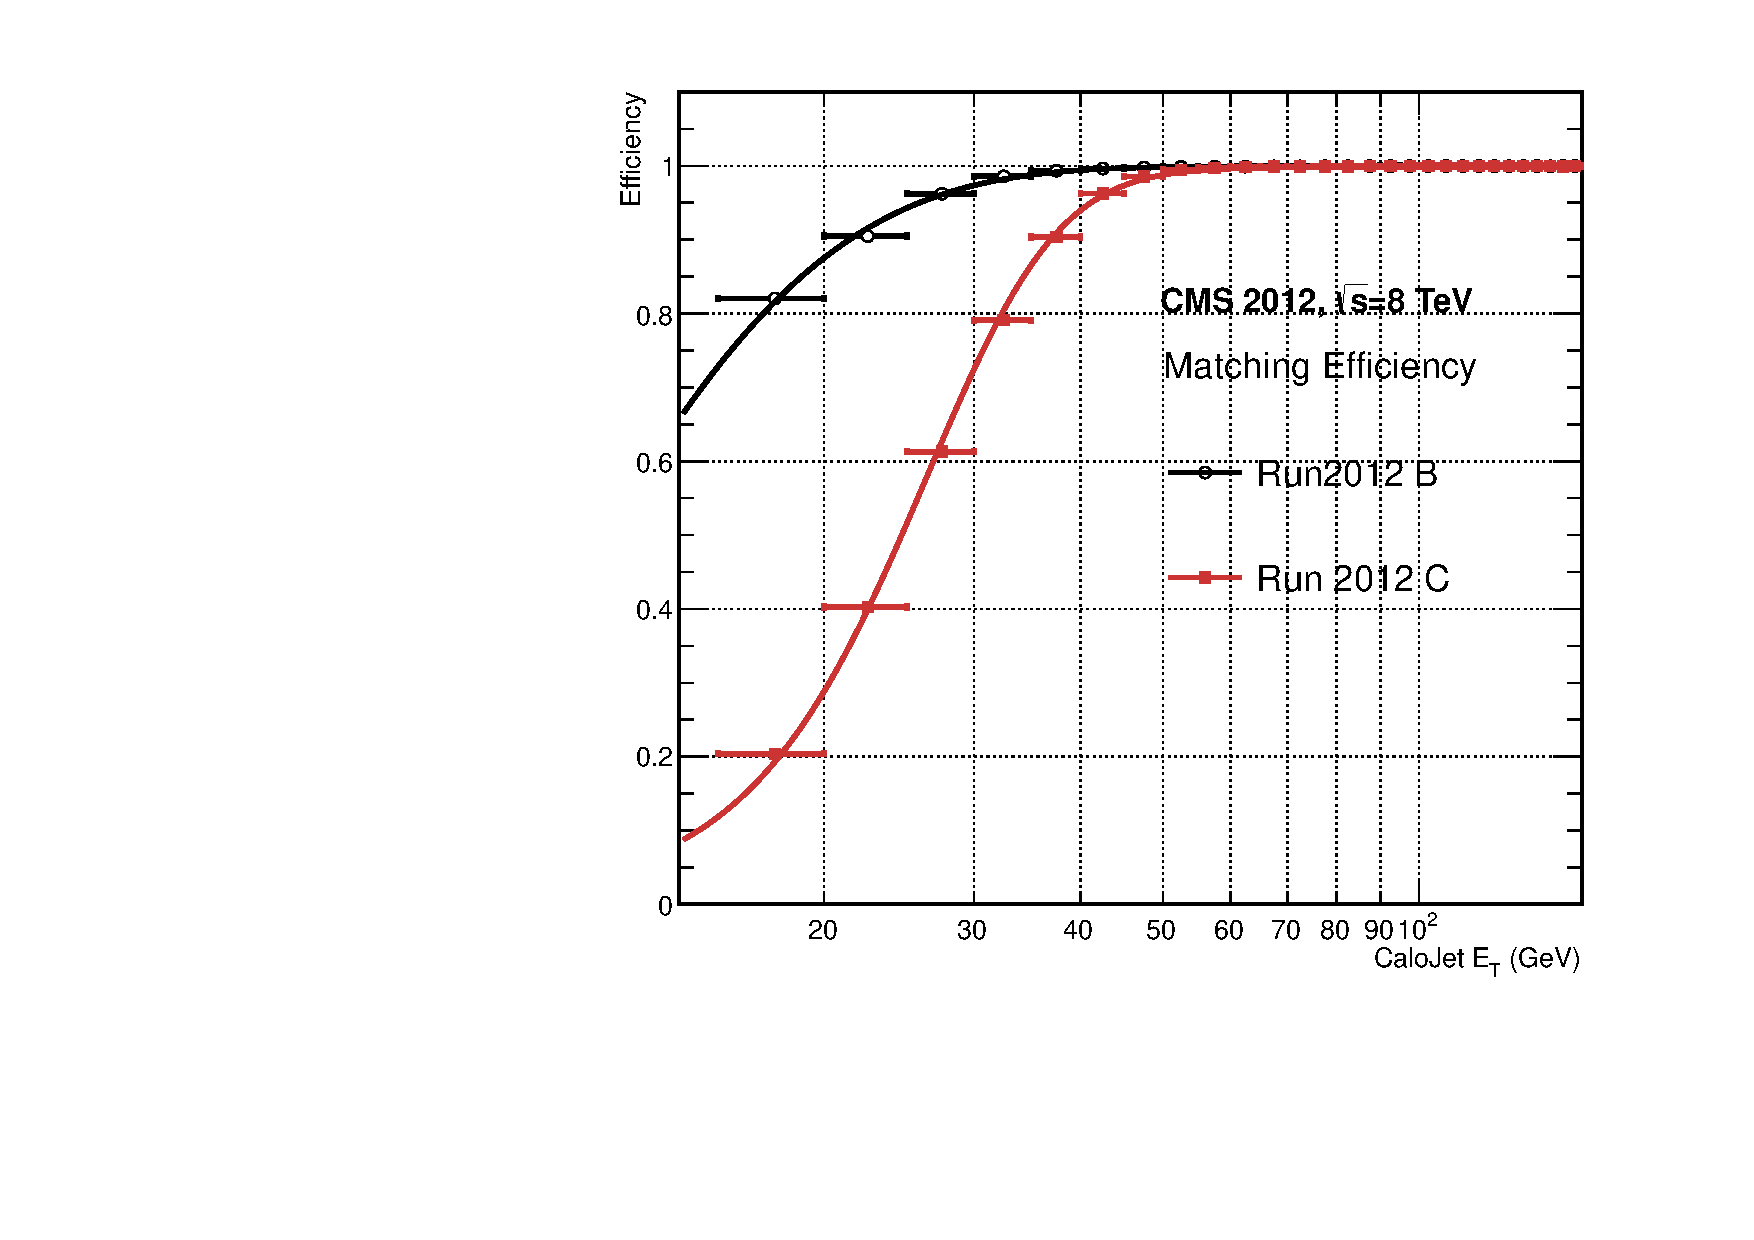
\includegraphics{plots/leadjet_matchingeff.pdf}}
\caption[Leading jet matching efficiency as a function of the offline CaloJet $\et$.]{Leading jet matching efficiency as a function of the offline CaloJet $\et$, measured in an isolated muon triggered dataset in the 2012B and 2012C run periods.}
  \label{fig:leadjetmatcheff}
\end{figure}

It can be seen that the turn on is sharper during the 2012B run
period. The seed threshold requirement of a 5 \GeV jet seed in run 2012C results
in more events in which even the lead offline jet does not have an associated L1 jet. For larger jet $\et$
thresholds, typical of thresholds used in physics analyses, 100$\%$ efficiency is observed.

The matching efficiencies have a $\mu$ values of 6.62 GeV and 19.51 GeV for Run 2012B and 2012C respectively and is shown in Table~\ref{tab:matcheff}. 

\begin{table}
\begin{center}
\begin{tabular*}{0.5\textwidth}{|c|c|c|}
\cline{1-3}
Run Period & $\mu$ & $\sigma$ \\ \cline {1-3}
2012B & 6.62 $\pm$ 0.01 & 0.79 $\pm$ 0.03  \\ \cline{1-3}
2012C & 19.51 $\pm$ 0.03 & 7.14 $\pm$ 0.02 \\ \cline{1-3}
\end{tabular*}
\caption[Results of a cumulative EMG function fit to the turn-on
curves for the matching efficiency of the leading jet in an event to
a Level-1 jet in run 2012C and 2012B data.]{Results of a cumulative EMG function fit to the turn-on
curves for the matching efficiency of the leading jet in an event to
a Level-1 jet in run 2012C and 2012B data, measured in an isolated
muon triggered sample. The turn-on point, $\mu$, and resolution, $\sigma$, are measured with respect to offline Calo Jet $\et$.} \label{tab:matcheff}
\end{center}
\end{table}

\section{Leading Jet Energy Resolution}
\label{app:jetpuresolution}

\begin{figure}[htp]

    \centering
    \subfloat[]{  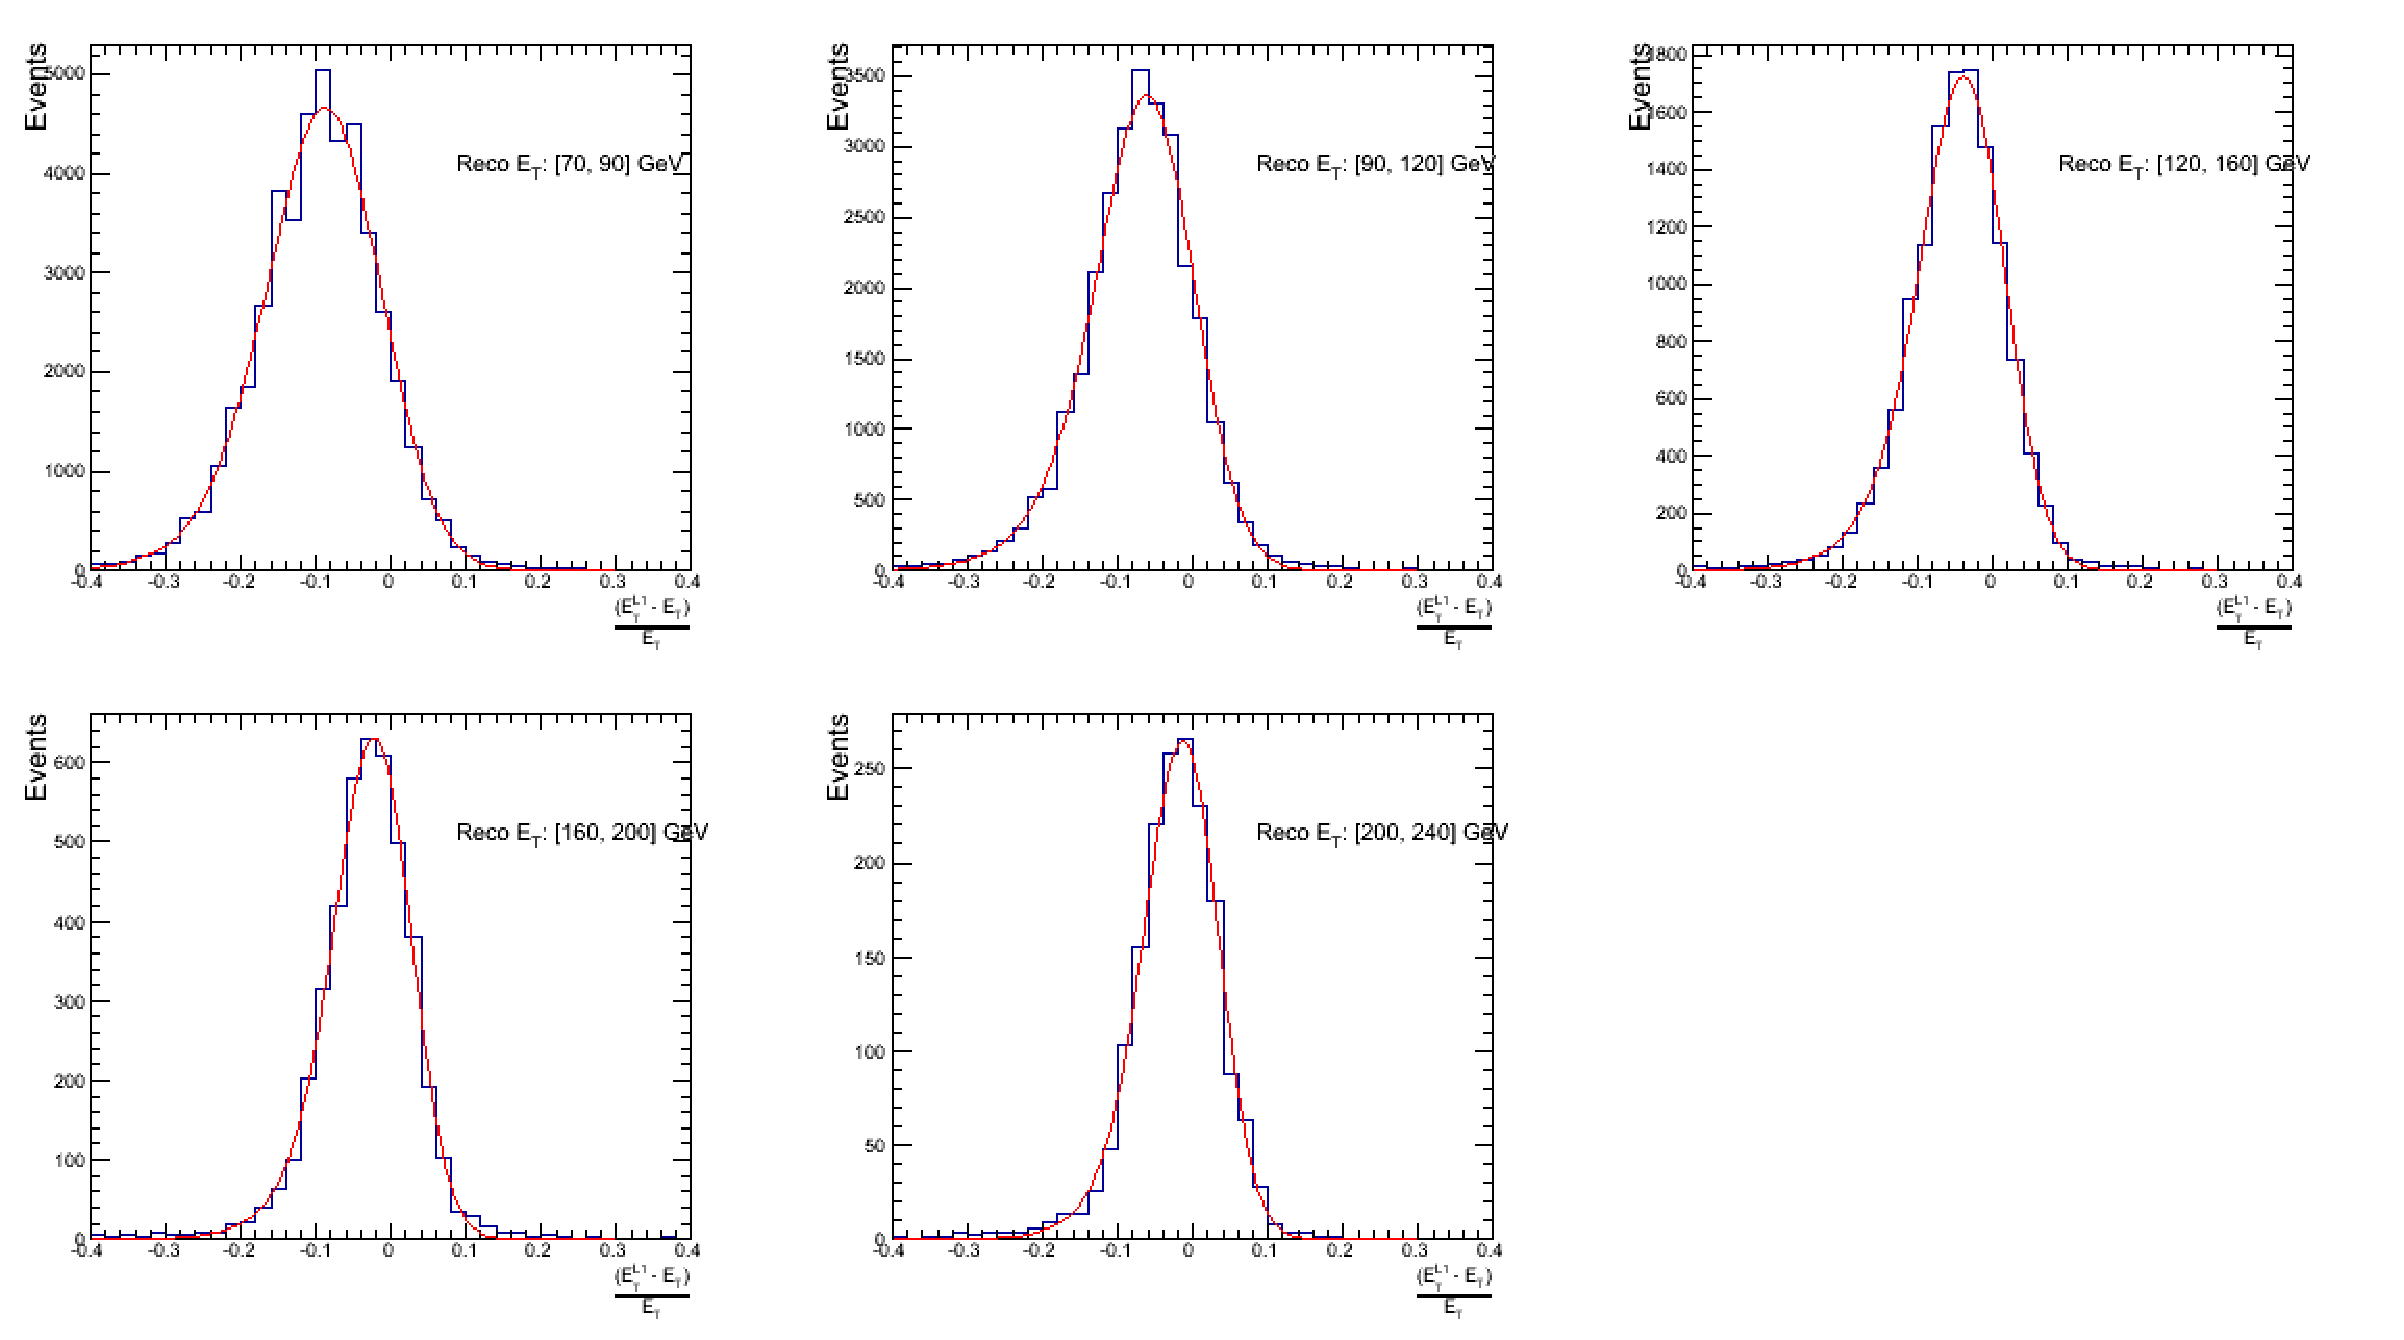
\includegraphics[width=0.95\textwidth]{plots/ptresolution_low.pdf}  }\,
    %\caption{}
\end{figure}

\begin{figure}
    %\ContinuedFloat
    \centering
    \subfloat[]{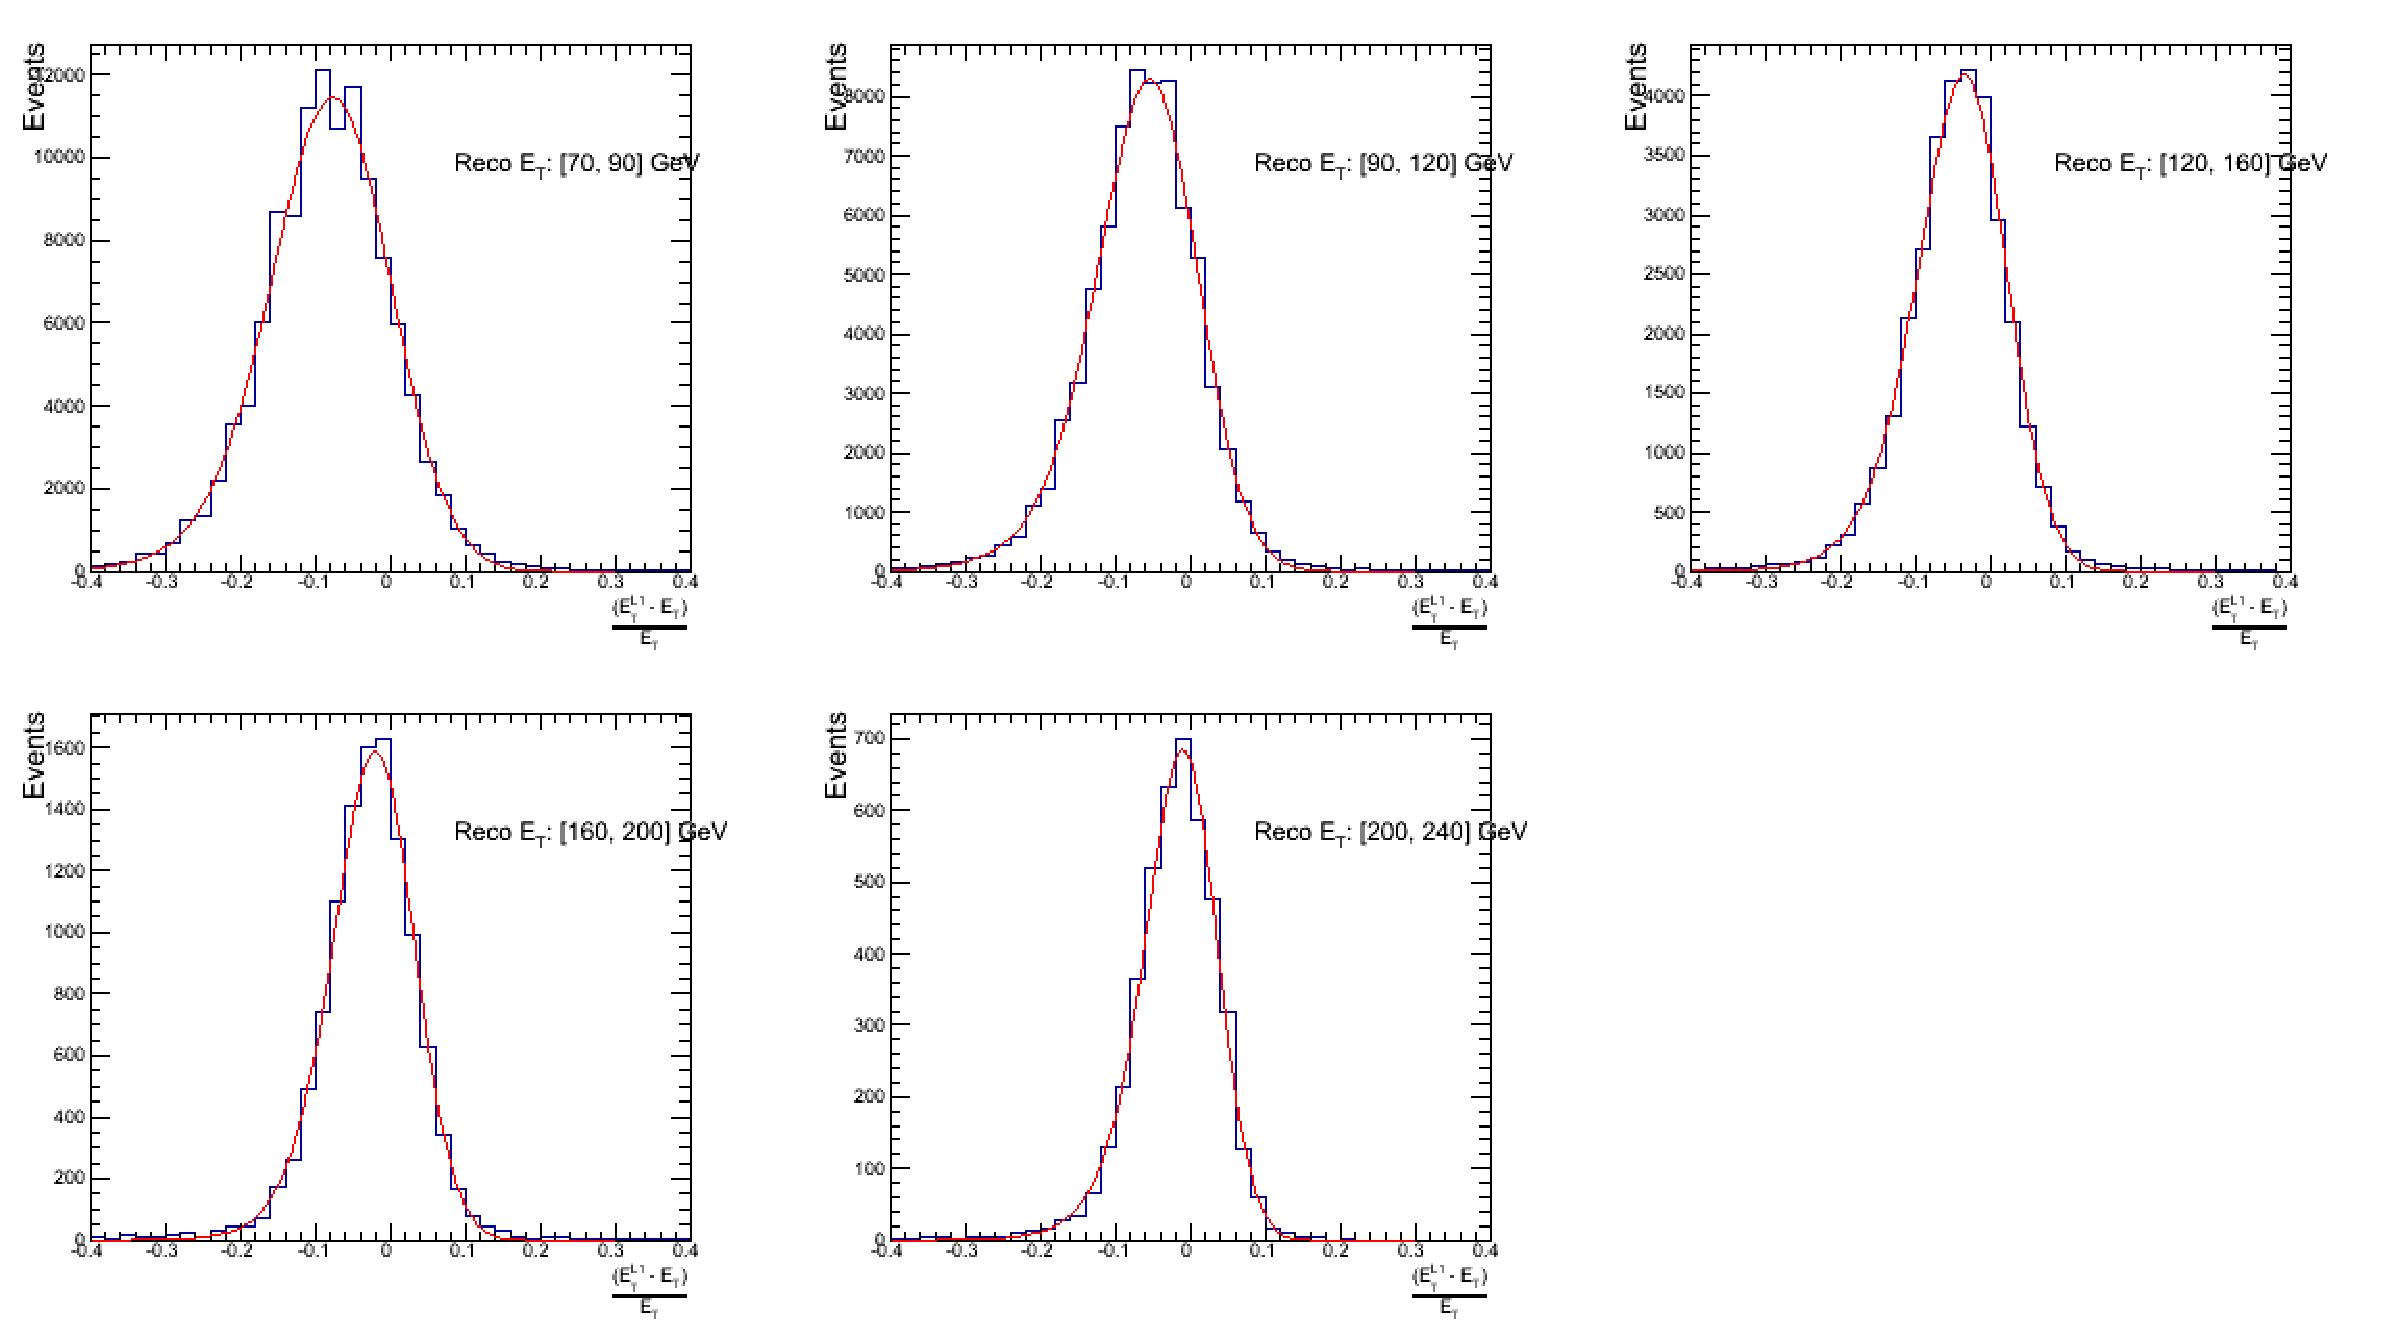
\includegraphics[width=0.95\textwidth]{plots/ptresolution_medium.pdf}}\,
    \subfloat[]{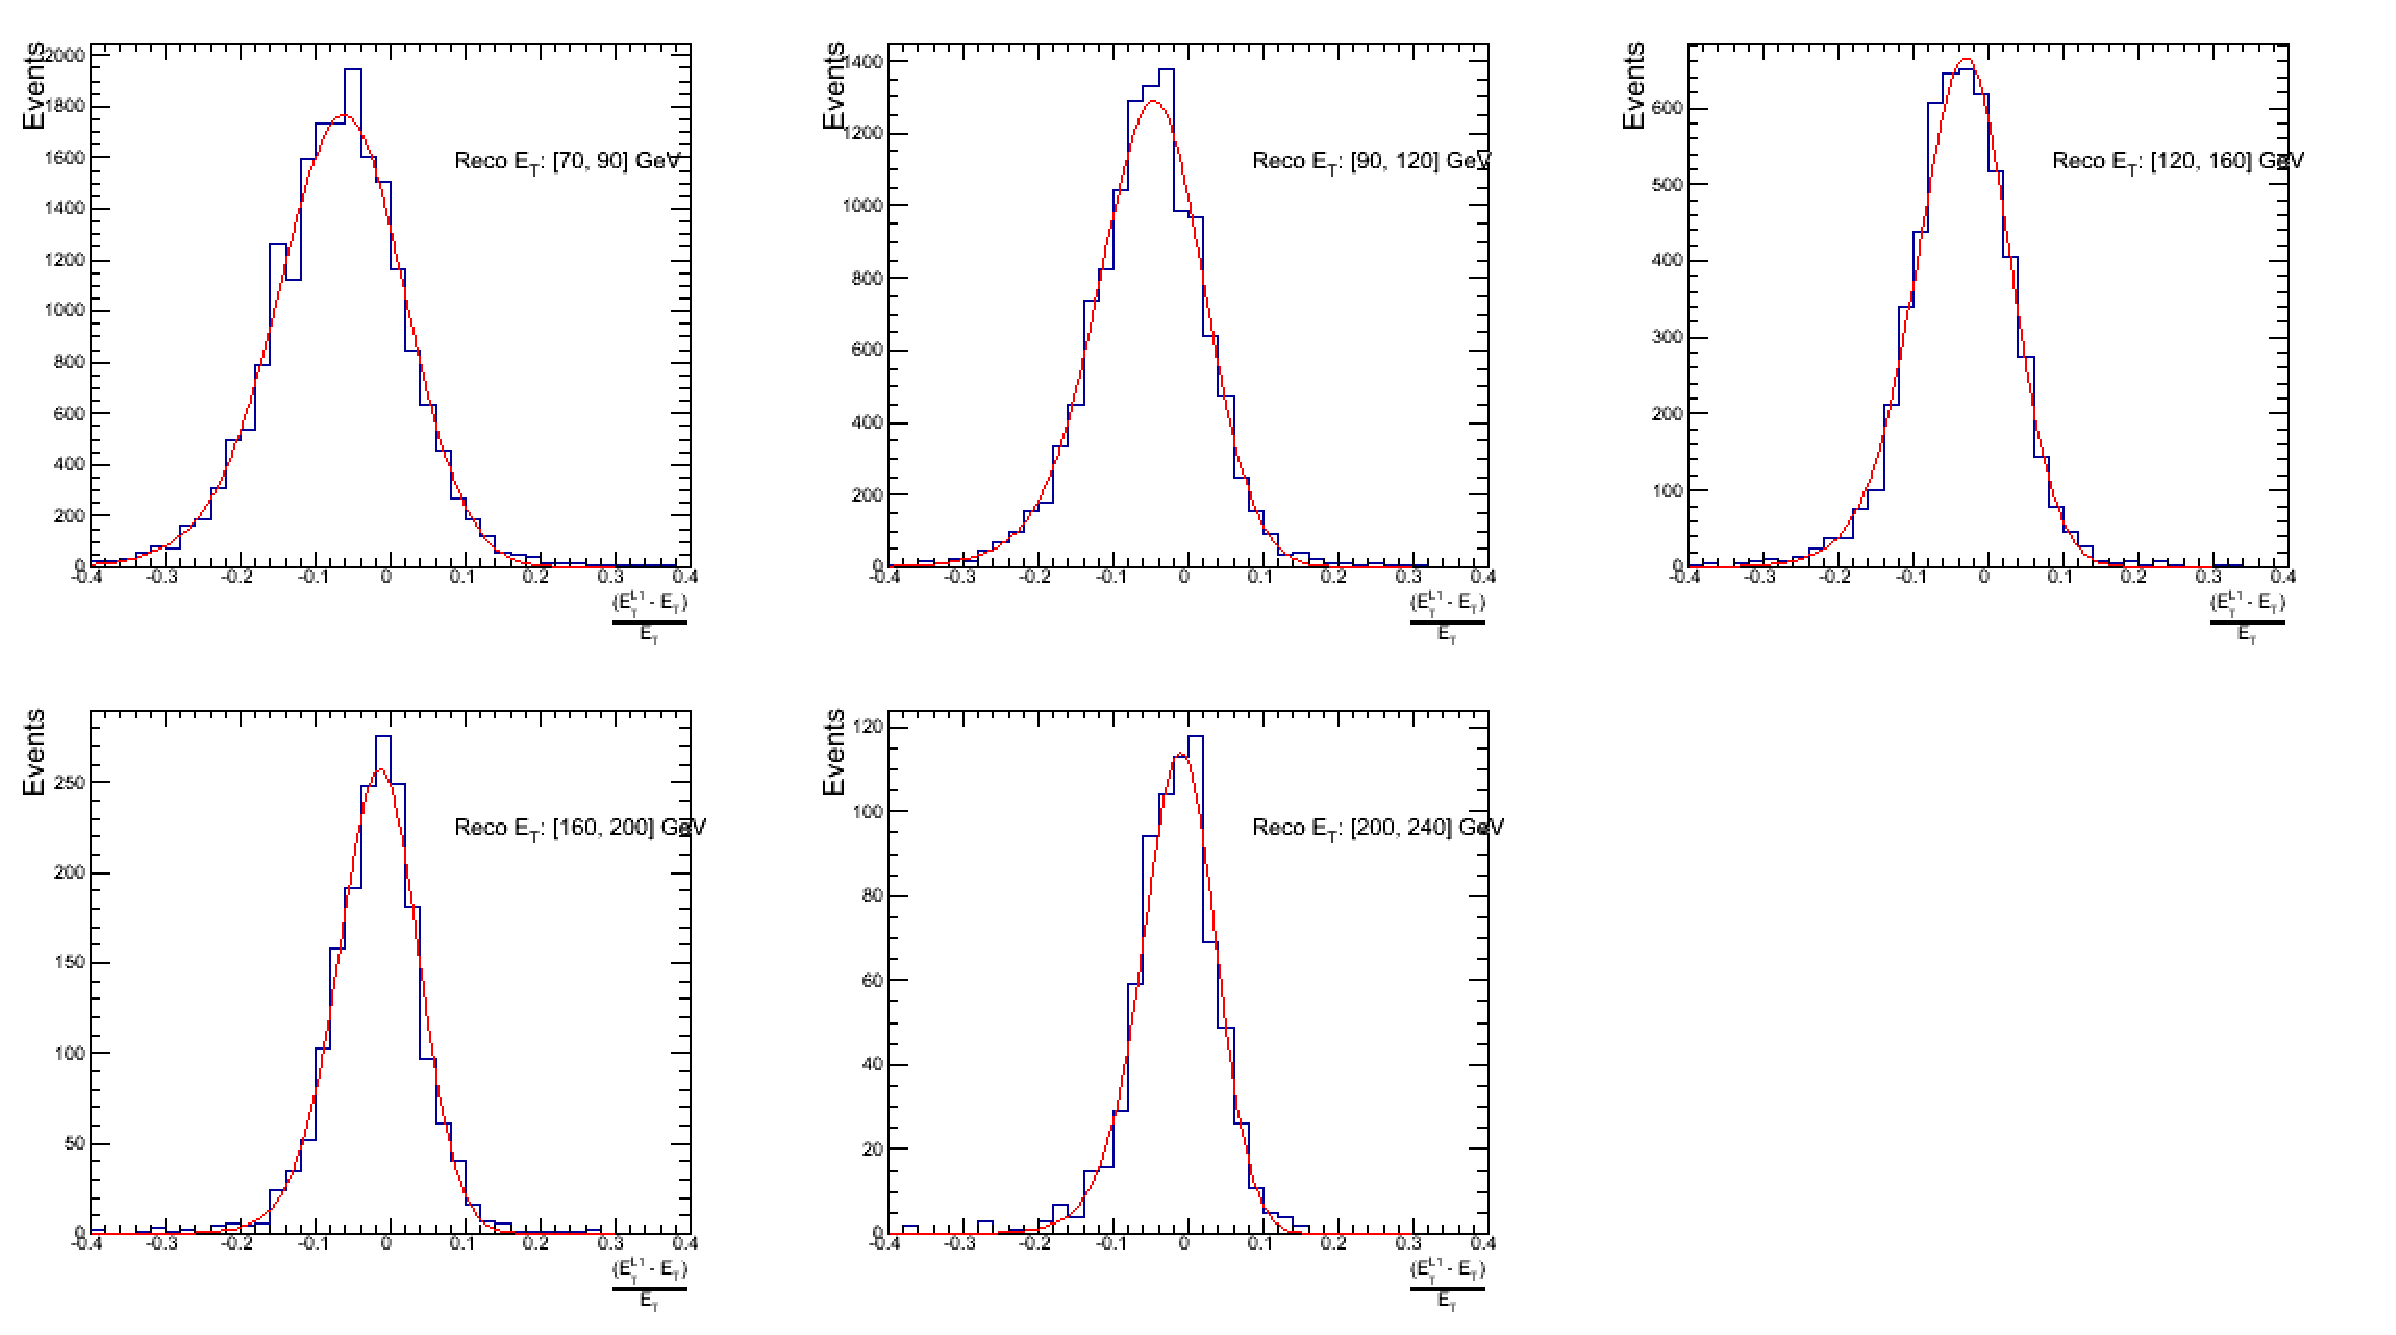
\includegraphics[width=0.95\textwidth]{plots/ptresolution_high.pdf}}\,

      \caption[ Resolution plots of the leading offline \Calo $\et$ measured as a function of  $\frac{(\text{L1 E}_{T} -  \text{Offline E}_{T})}{\text{Offline E}_{T}}$ for  low (a), medium (b) and high (c) pile-up conditions.] { Resolution plots of the leading offline jet \Calo $\et$ measured as a function of  $\frac{(\text{L1 E}_{T} -  \text{Offline E}_{T})}{\text{Offline E}_{T}}$ for  low (a), medium (b) and high (c) pile-up conditions. }
\end{figure}

\begin{figure}[htpb]

    \centering
    \subfloat[]{  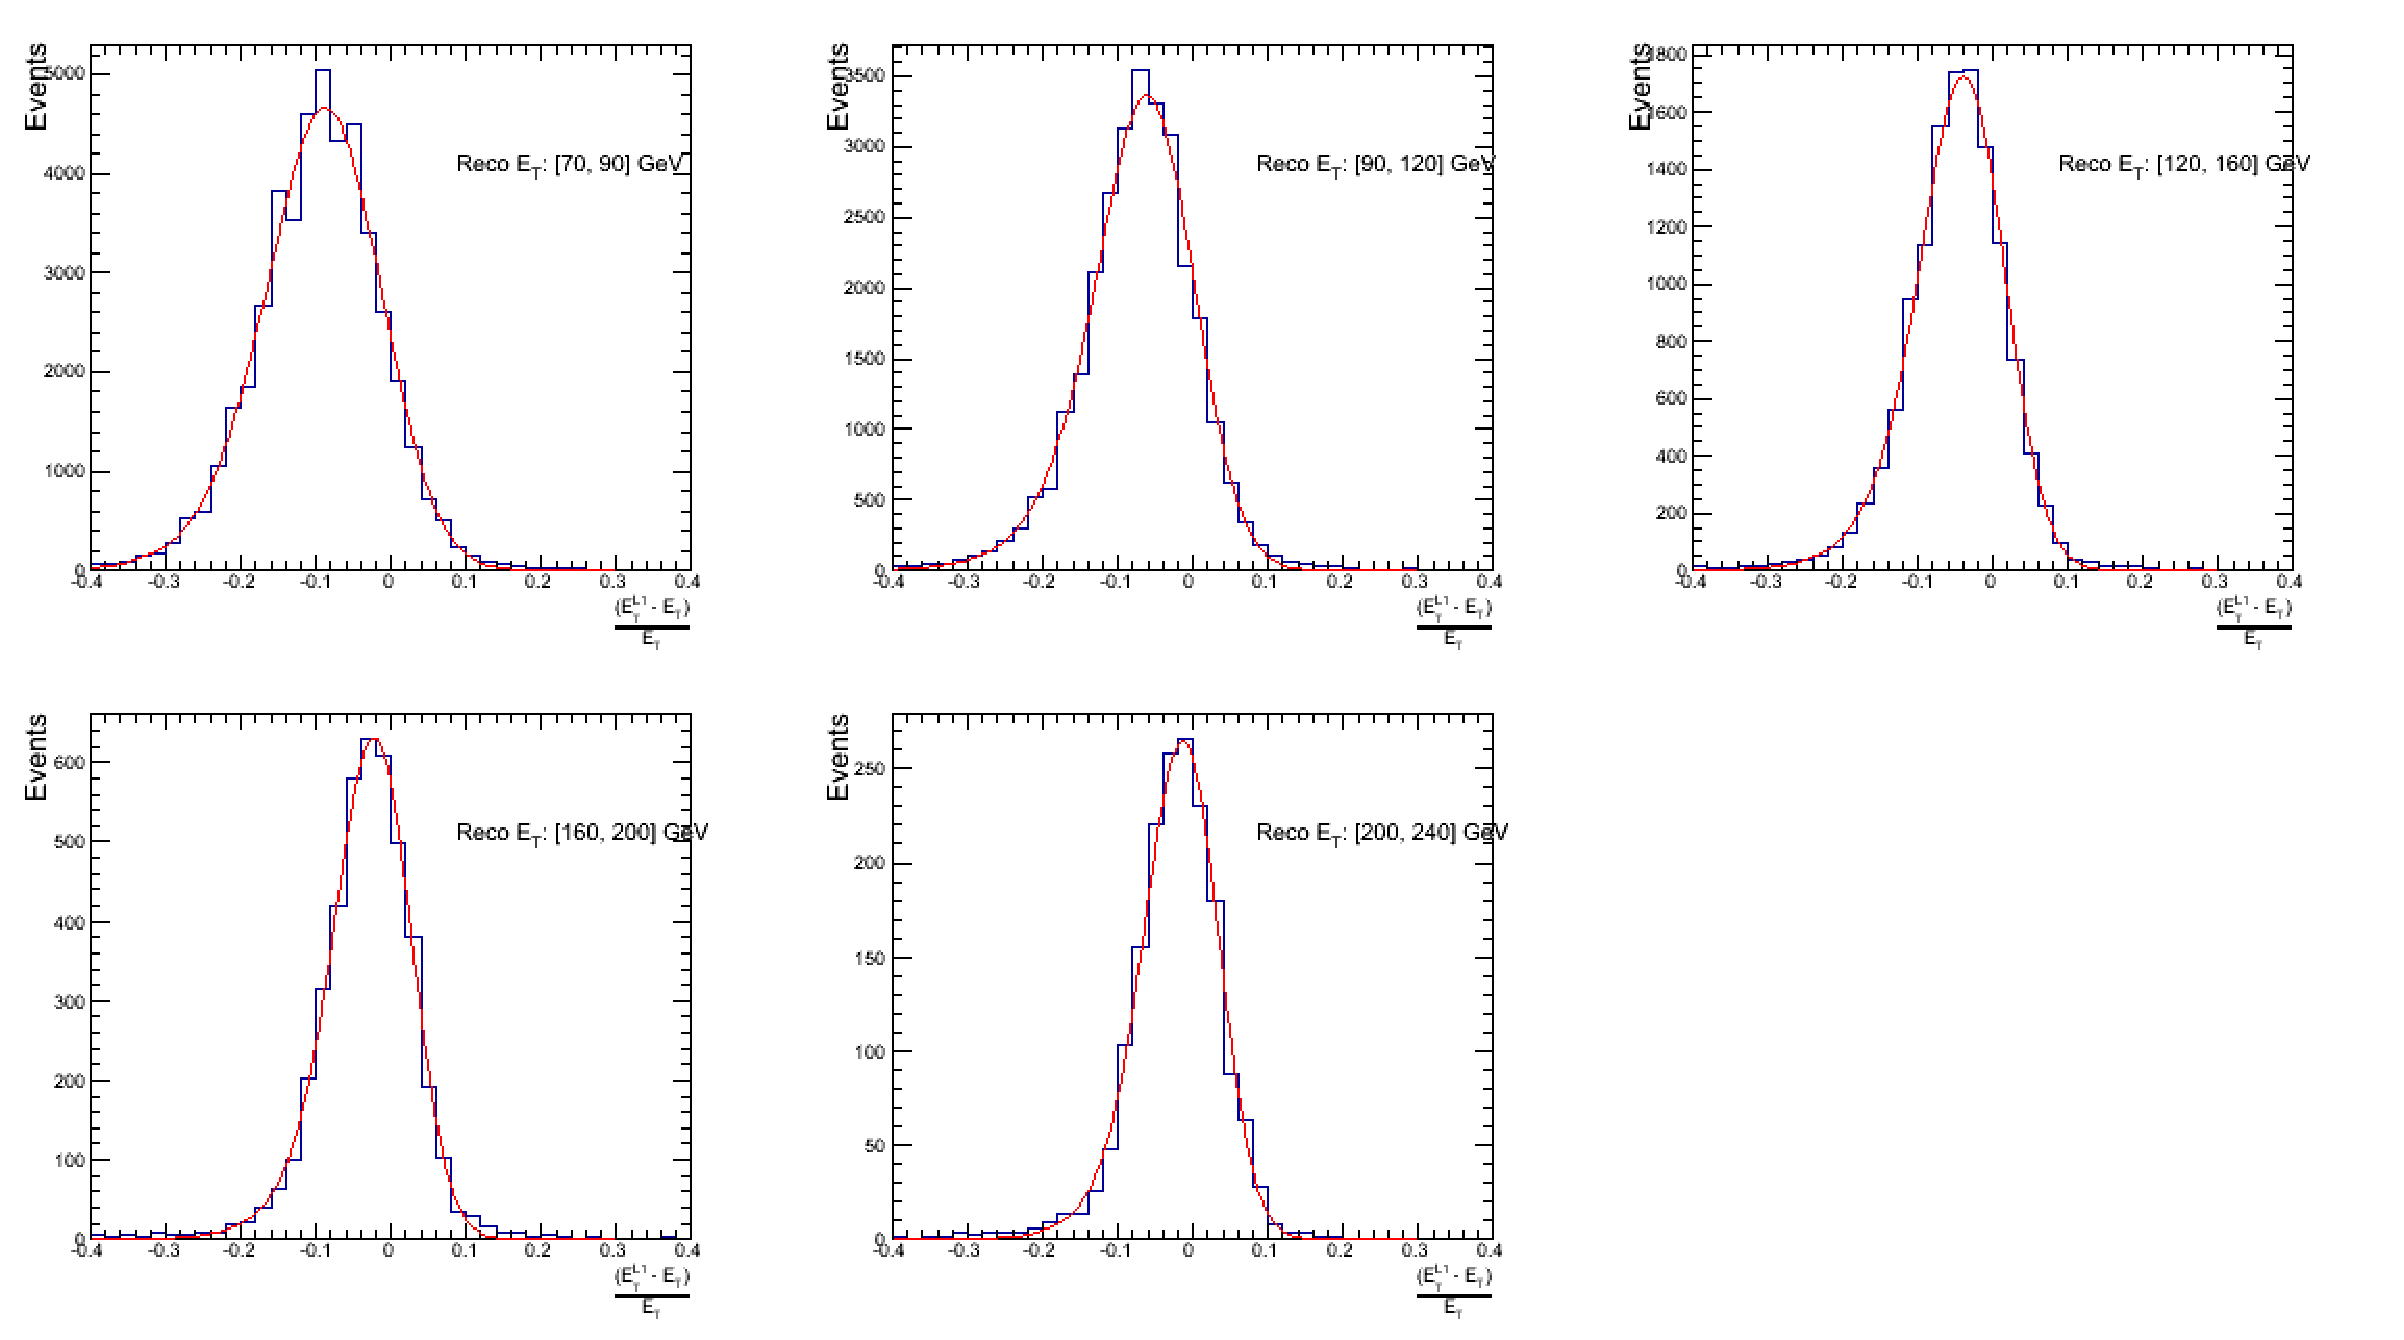
\includegraphics[width=0.95\textwidth]{plots/ptresolution_low.pdf}  }\,
    \subfloat[]{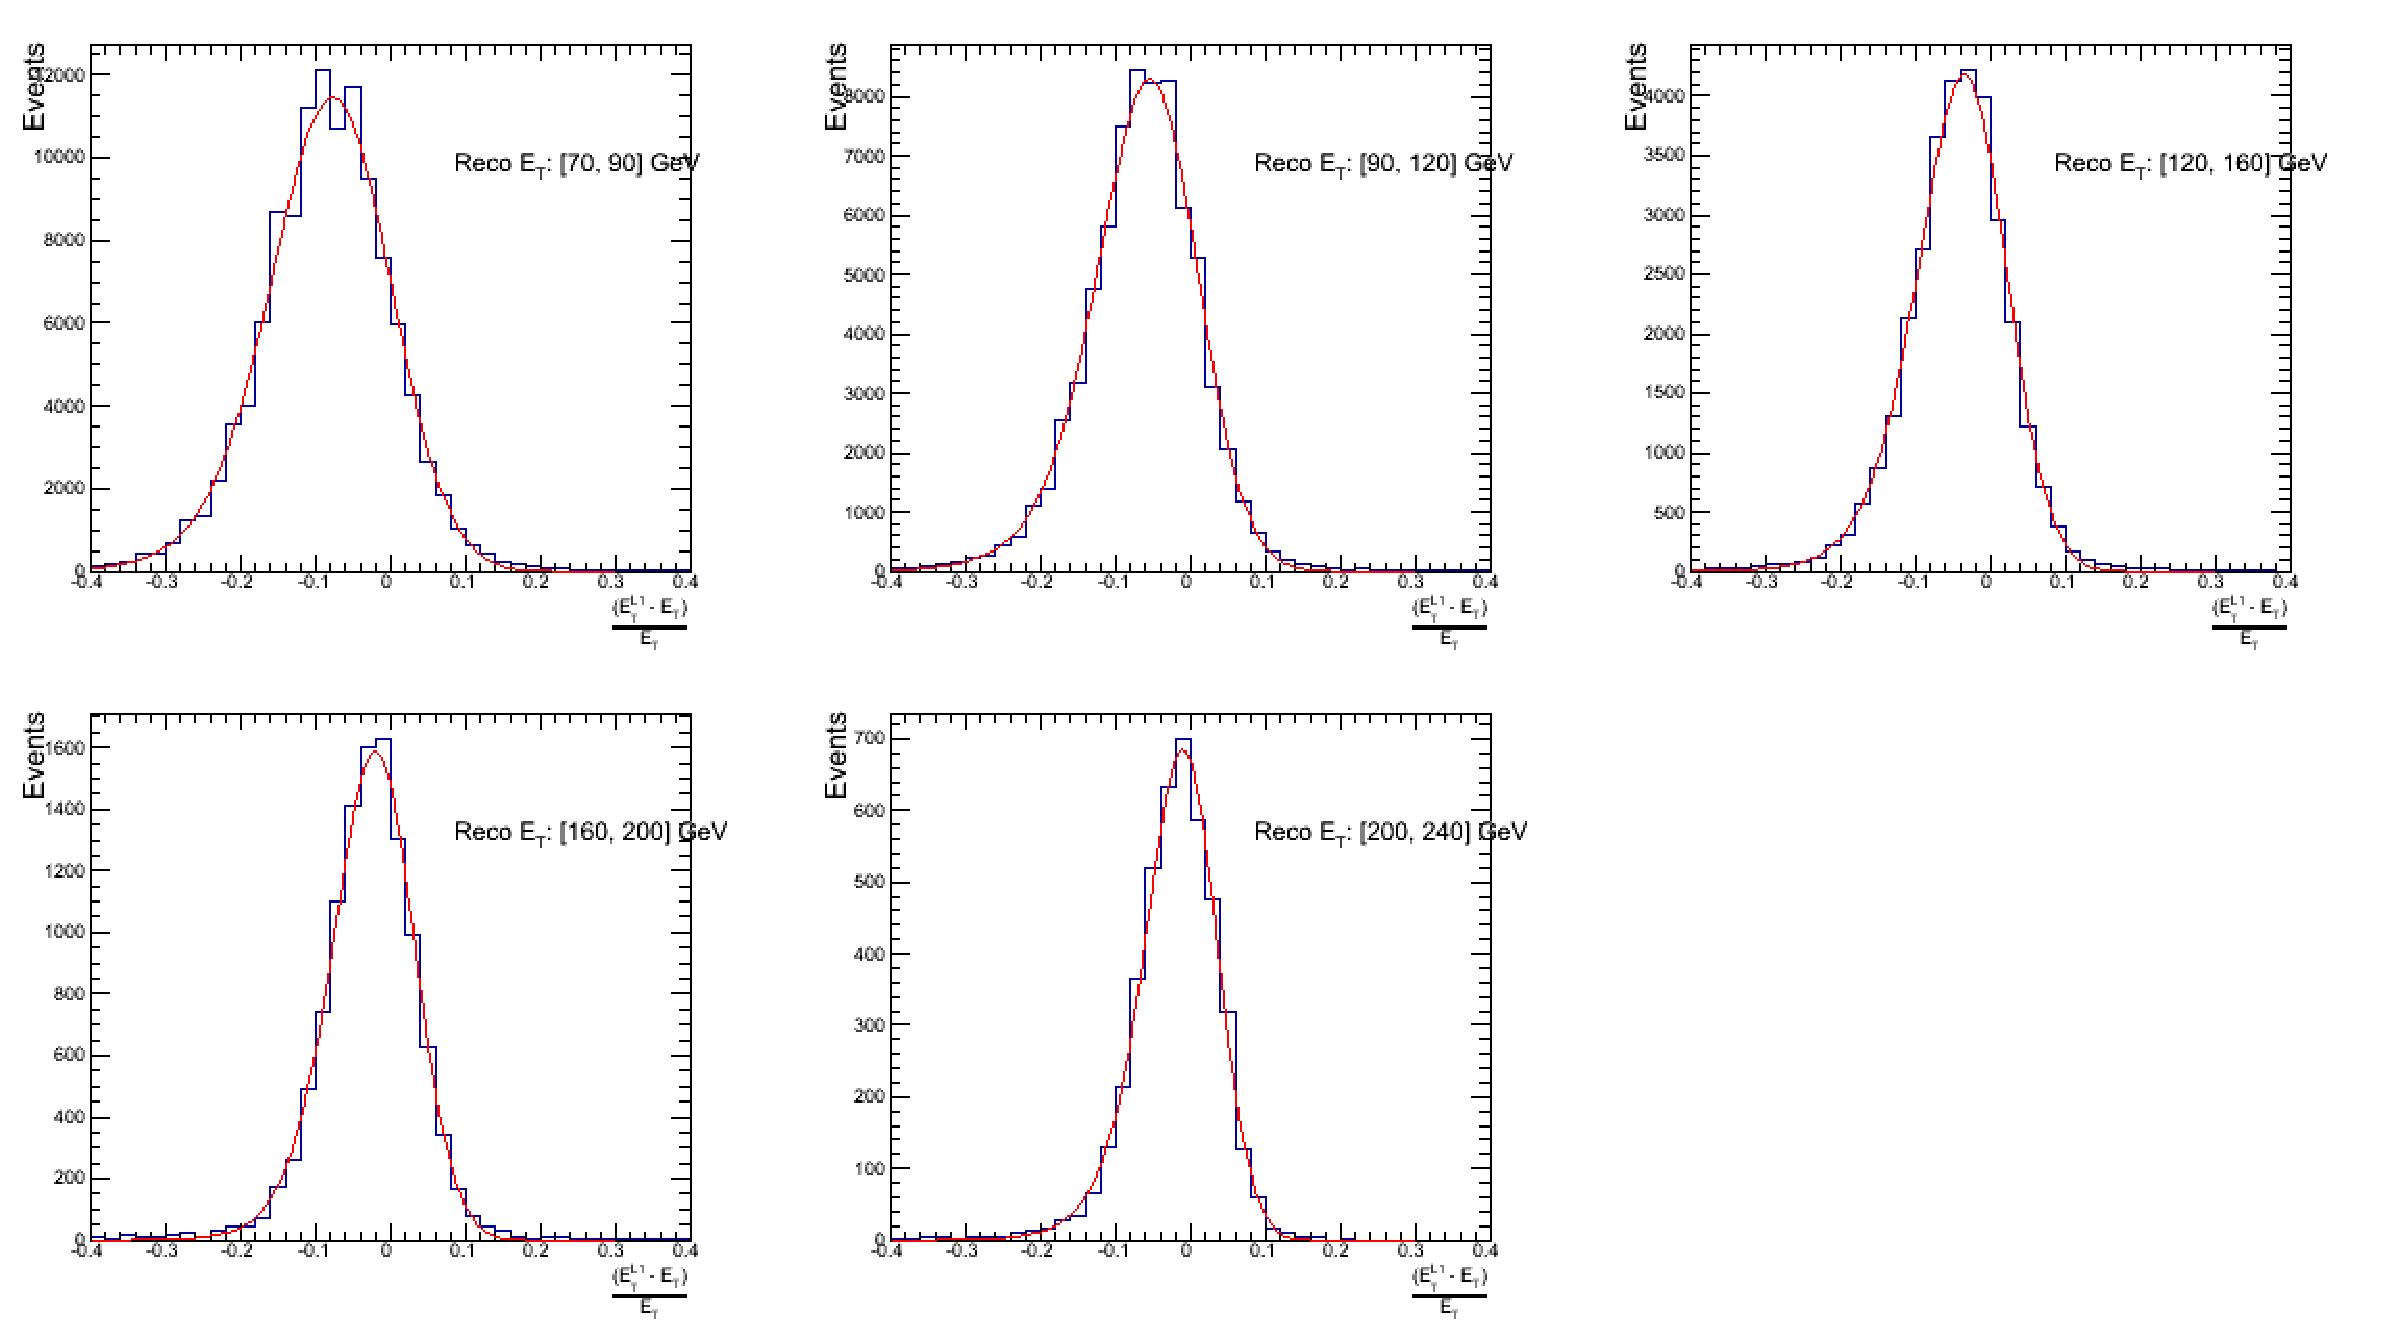
\includegraphics[width=0.95\textwidth]{plots/ptresolution_medium.pdf}}\,

\end{figure}

\begin{figure}
   % \ContinuedFloat
    \centering
    \subfloat[]{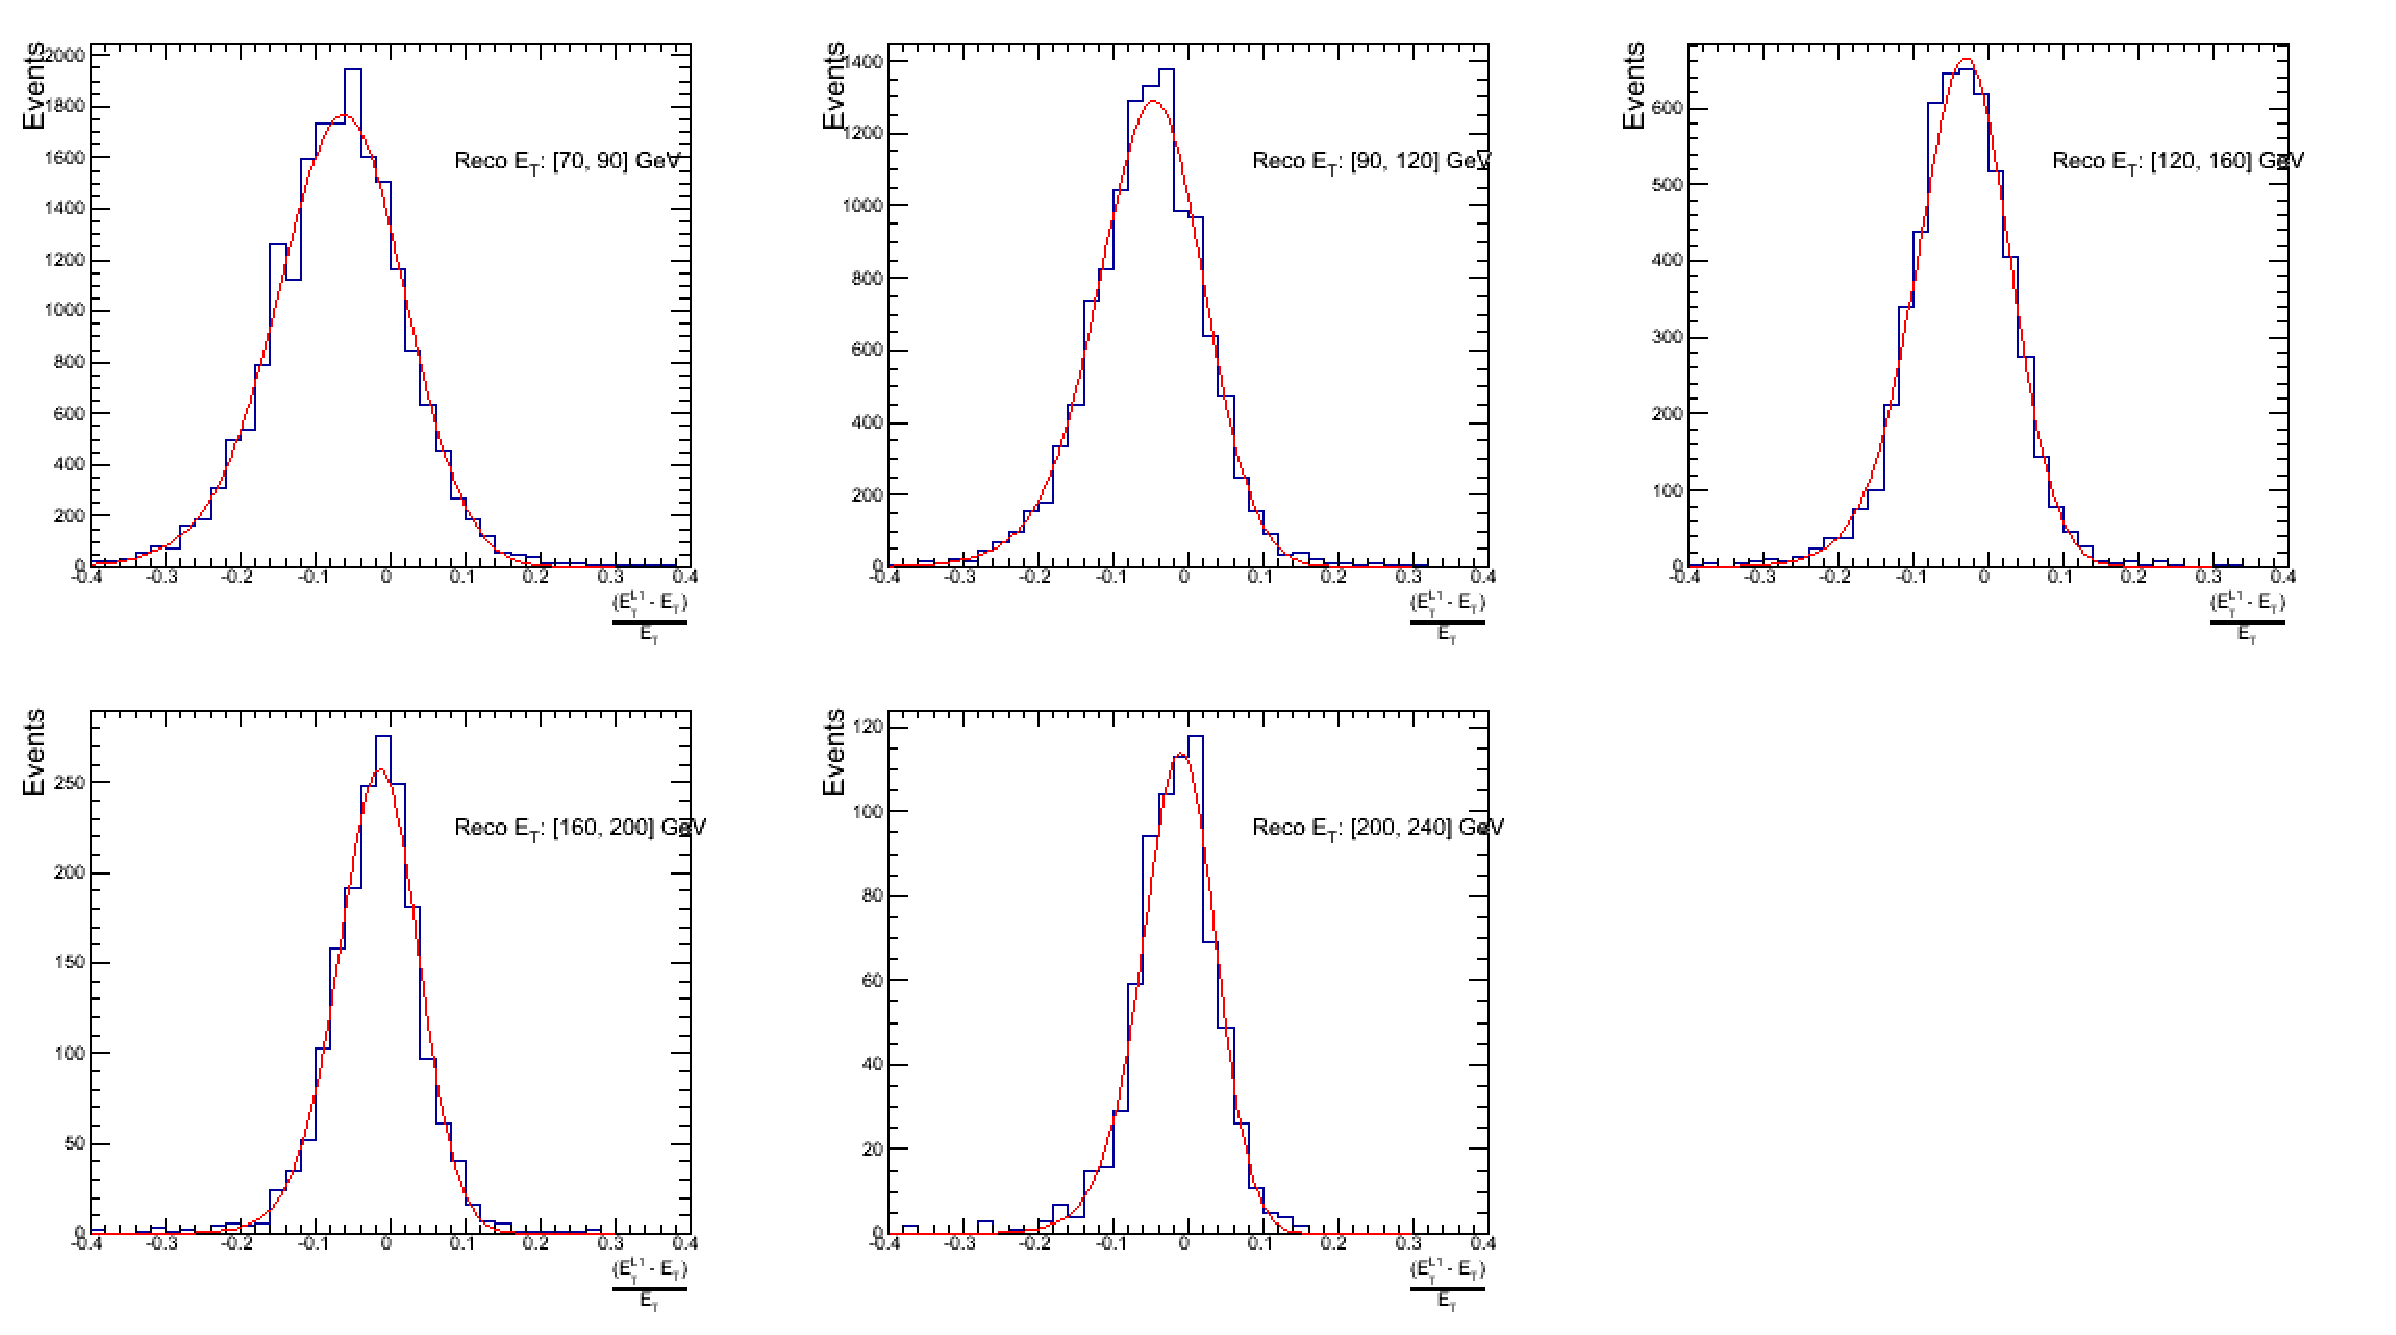
\includegraphics[width=0.95\textwidth]{plots/ptresolution_high.pdf}}\,

      \caption[ Resolution plots of the leading off-line PF $\et$ measured as a function of  $\frac{(\text{L1 E}_{T} -  \text{Offline E}_{T})}{\text{Offline E}_{T}}$ for  low (a), medium (b) and high (c) pile-up conditions.] { Resolution plots of the leading offline jet \PF $\et$ measured as a function of  $\frac{(\text{L1 E}_{T} -  \text{Offline E}_{T})}{\text{Offline E}_{T}}$ for  low (a), medium (b) and high (c) pile-up conditions. }
  
\end{figure}


\newpage
\section{Resolution for Energy Sum Quantities}
\label{app:jetenergysums}

The following plots show the resolution parameters for the four energy sum quantities as a function of the quantity (q) itself. In this case, The mean and RMS of the individual $\frac{(\text{L1 q} -  \text{Offline q})}{\text{Offline q}}$ distributions, in bins of the quantity q is displayed. 

\begin{figure}[h!]
  \vspace{20pt}
        \centering
        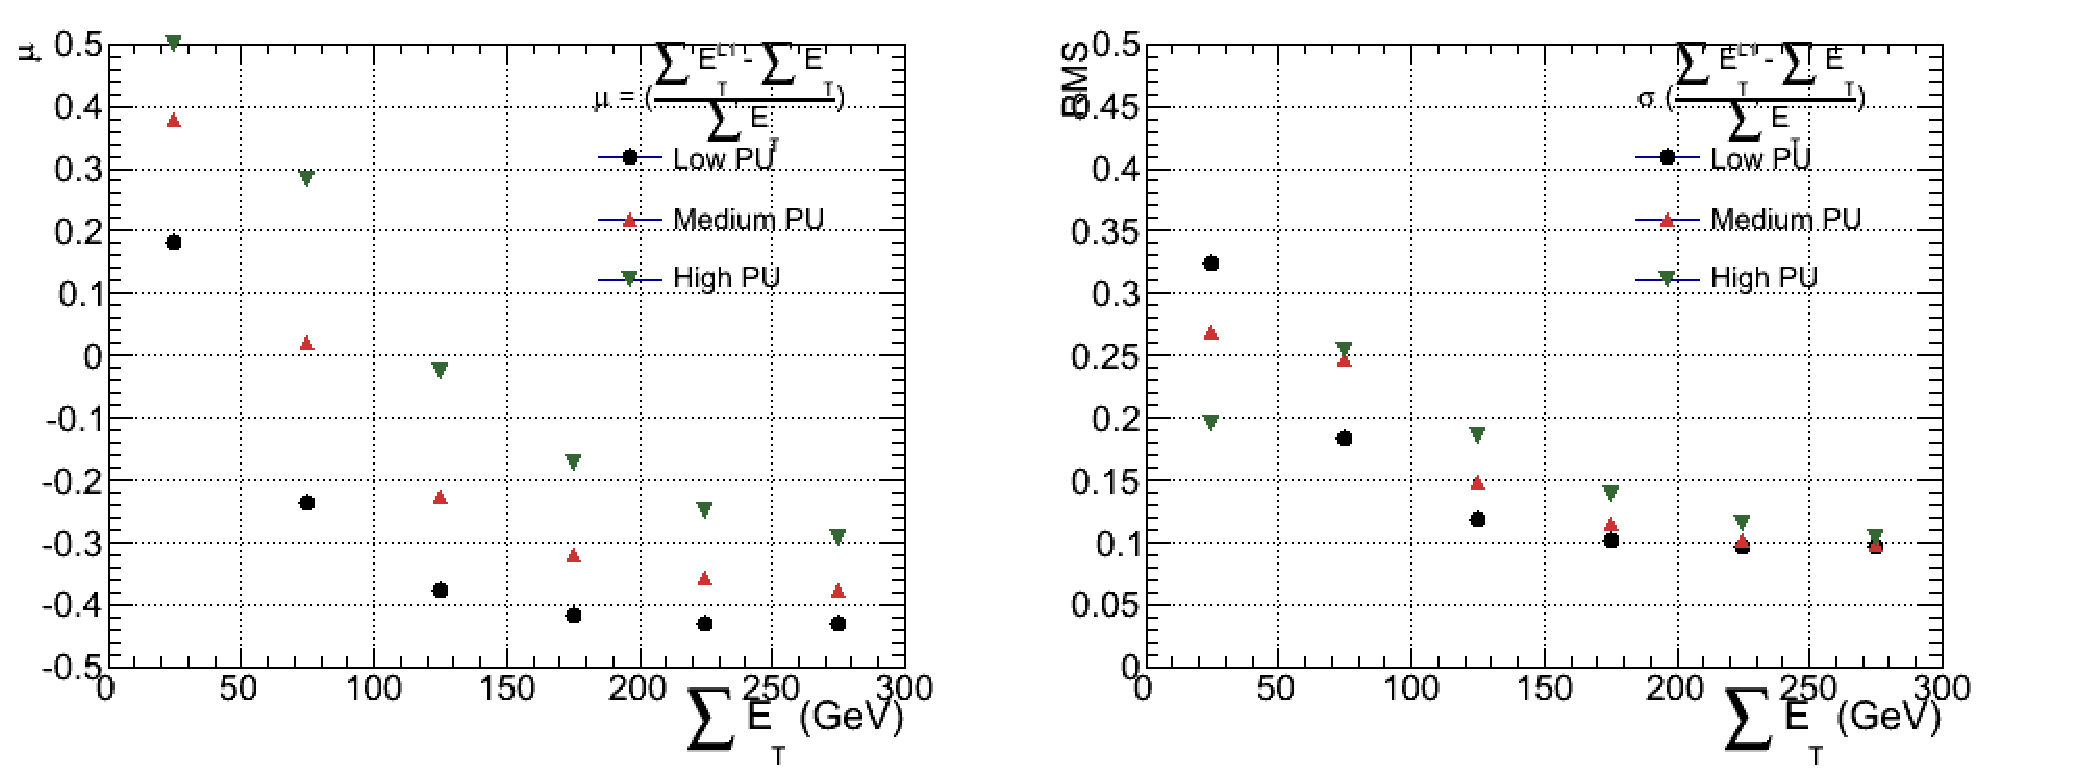
\includegraphics[width=1.0\textwidth]{plots/res_CaloSumET_summary.pdf}
        \caption[$\sum$ $\et$~resolution parameters in bins of Calo $\sum E_{T}$  measured for the defined low, medium and high pile up conditions.]{$\sum$ $\et$~resolution parameters in bins of Calo $\sum E_{T}$  measured for the defined low, medium and high pile up conditions. The plots show the mean $\mu$ (left), resolution $\sigma$ (RMS) of the $\frac{\Delta q}{q}$ distributions.}
        \label{fig:caloetresultspu}
\end{figure}
\begin{figure}[h!]
  \vspace{20pt}
  \centering
        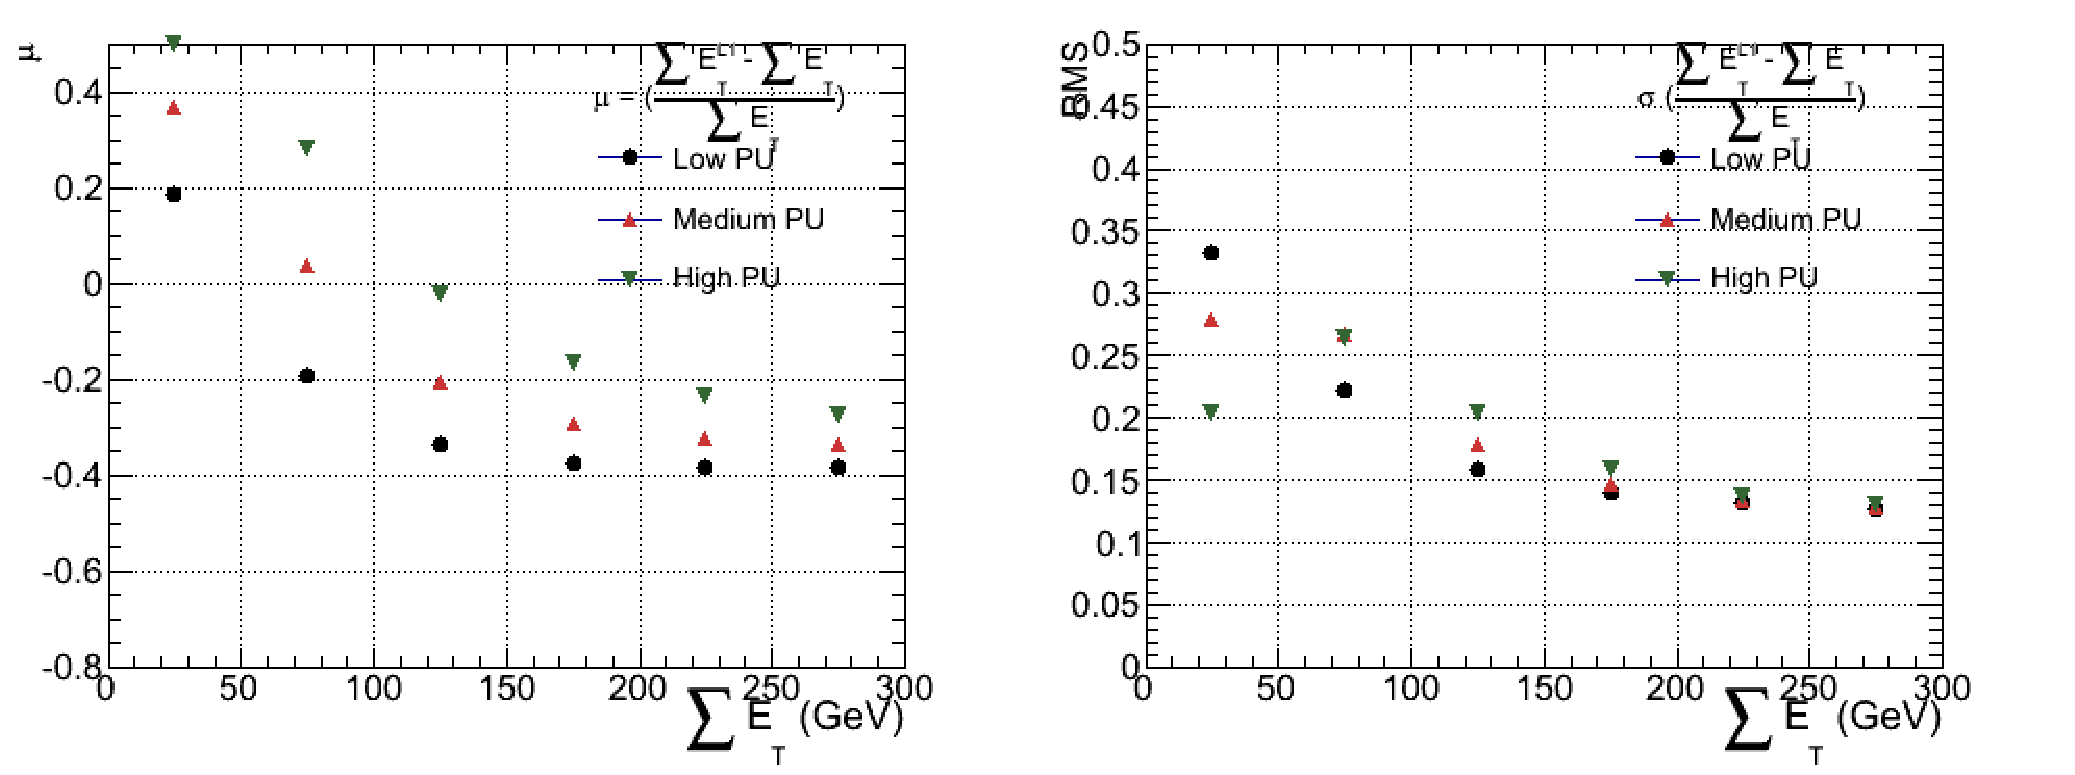
\includegraphics[width=1.0\textwidth]{plots/res_pfSumET_summary.pdf}
        \caption[$\sum$ $\et$~resolution parameters in bins of PF $\sum E_{T}$  measured for the defined low, medium and high pile up conditions. ]{$\sum$ $\et$~resolution parameters in bins of PF $\sum E_{T}$  measured for the defined low, medium and high pile up conditions. The plots show the mean $\mu$ (left), resolution $\sigma$ (RMS) of the $\frac{\Delta q}{q}$ distributions.}
        \label{fig:pfetresultspu}
\end{figure}

\begin{figure}[h!]
  \vspace{20pt}
        \centering
        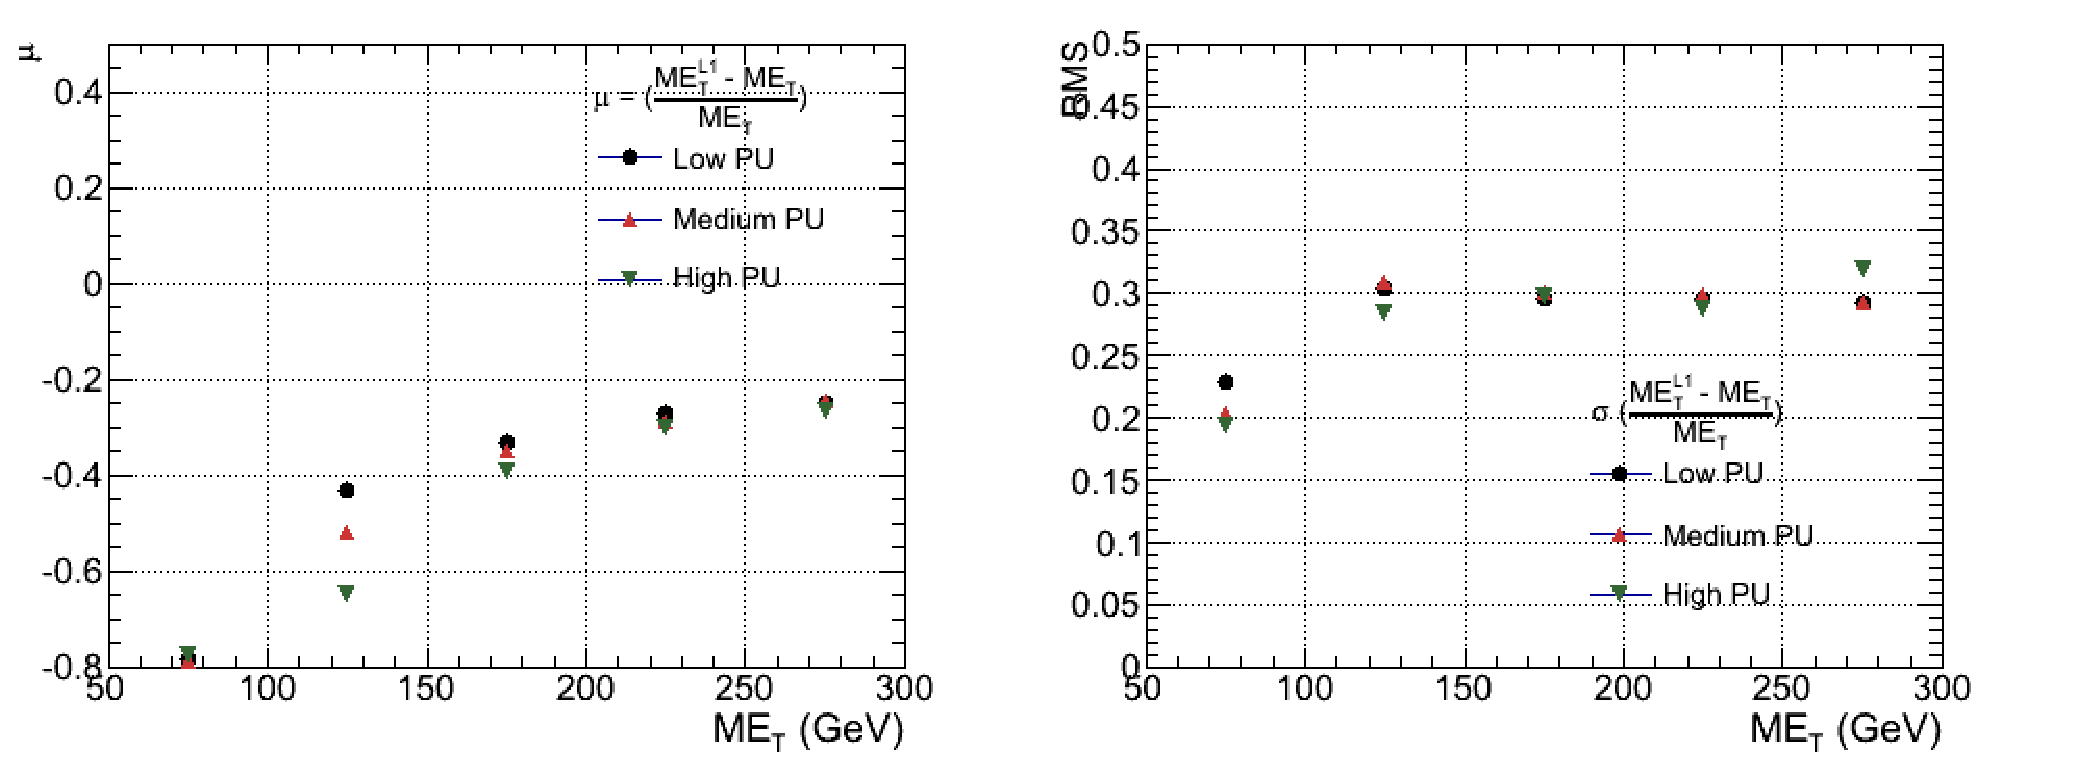
\includegraphics[width=1.0\textwidth]{plots/res_CaloMET_summary.pdf}
        \caption[$\met$~resolution parameters in bins of Calo $\met$~ measured for the defined low, medium and high pile up conditions.]{$\met$~resolution parameters in bins of Calo $\met$~ measured for the defined low, medium and high pile up conditions. The plots show the mean $\mu$ (left), resolution $\sigma$ (RMS) of the $\frac{\Delta q}{q}$  distributions.}
        \label{fig:calometresultspu}
\end{figure}
\begin{figure}[h!]
  \vspace{20pt}
        \centering
        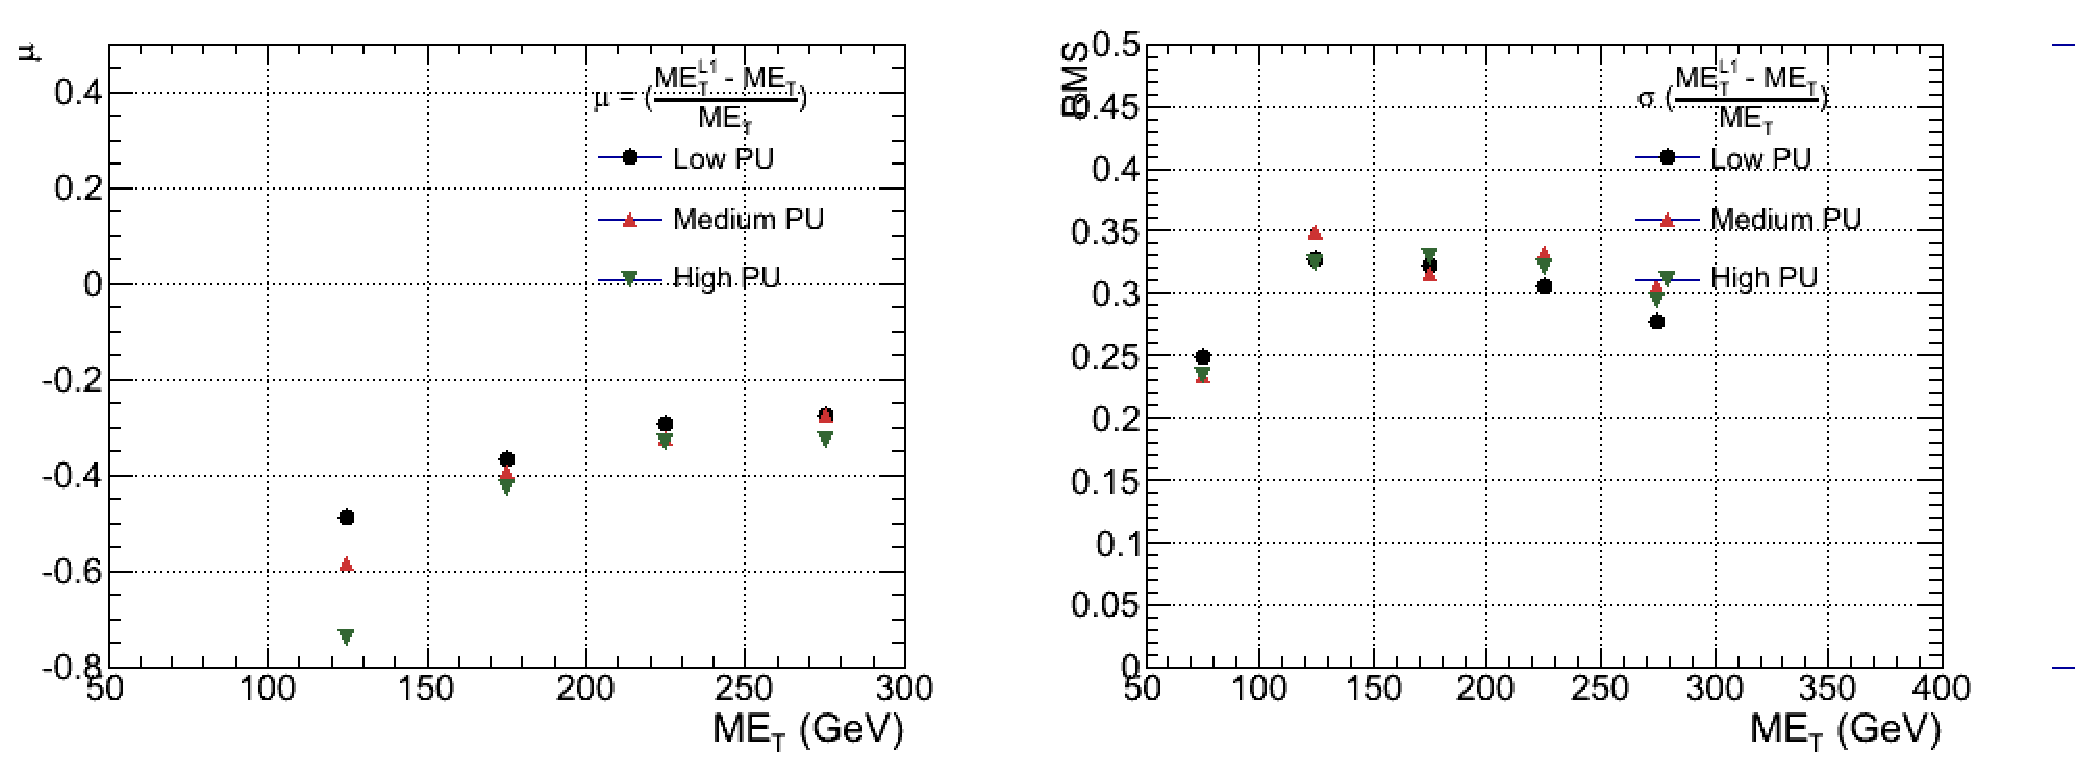
\includegraphics[width=1.0\textwidth]{plots/res_pfMET_summary.pdf}
        \caption[$\met$~resolution parameters in bins of PF $\met$~ measured for the defined low, medium and high pile up conditions.]{$\met$~resolution parameters in bins of PF $\met$~ measured for the defined low, medium and high pile up conditions. The plots show the mean $\mu$ (left), resolution $\sigma$ (RMS) of the $\frac{\Delta q}{q}$  distributions.}
        \label{fig:pfmetresultspu}
\end{figure}


\begin{figure}[h!]
  \vspace{20pt}
        \centering
        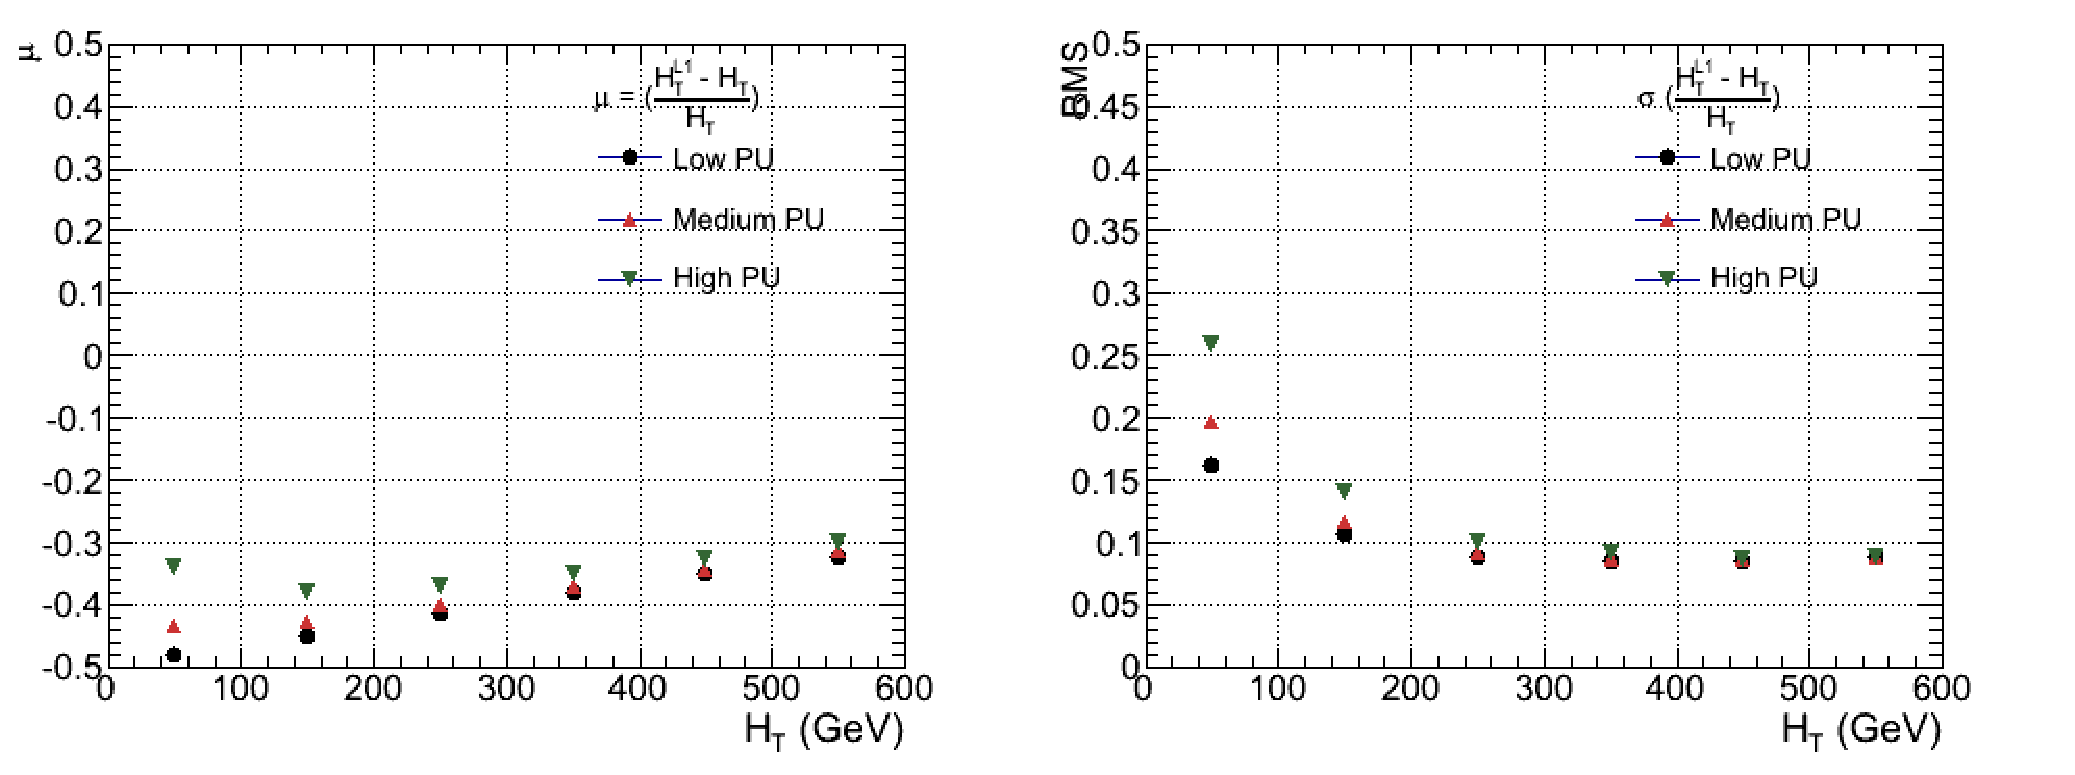
\includegraphics[width=1.0\textwidth]{plots/res_CaloHT_summary.pdf}
        \caption[$\theht$~resolution parameters in bins of Calo $\theht$~measured for the defined low, medium and high pile up conditions. ]{$\theht$~resolution parameters in bins of Calo $\theht$~measured for the defined low, medium and high pile up conditions. The plots show the mean $\mu$ (left), resolution $\sigma$ (RMS) of the $\frac{\Delta q}{q}$ distributions.}
        \label{fig:calohtresultspu}
\end{figure}
\begin{figure}[h!]
  \vspace{20pt}
        \centering
        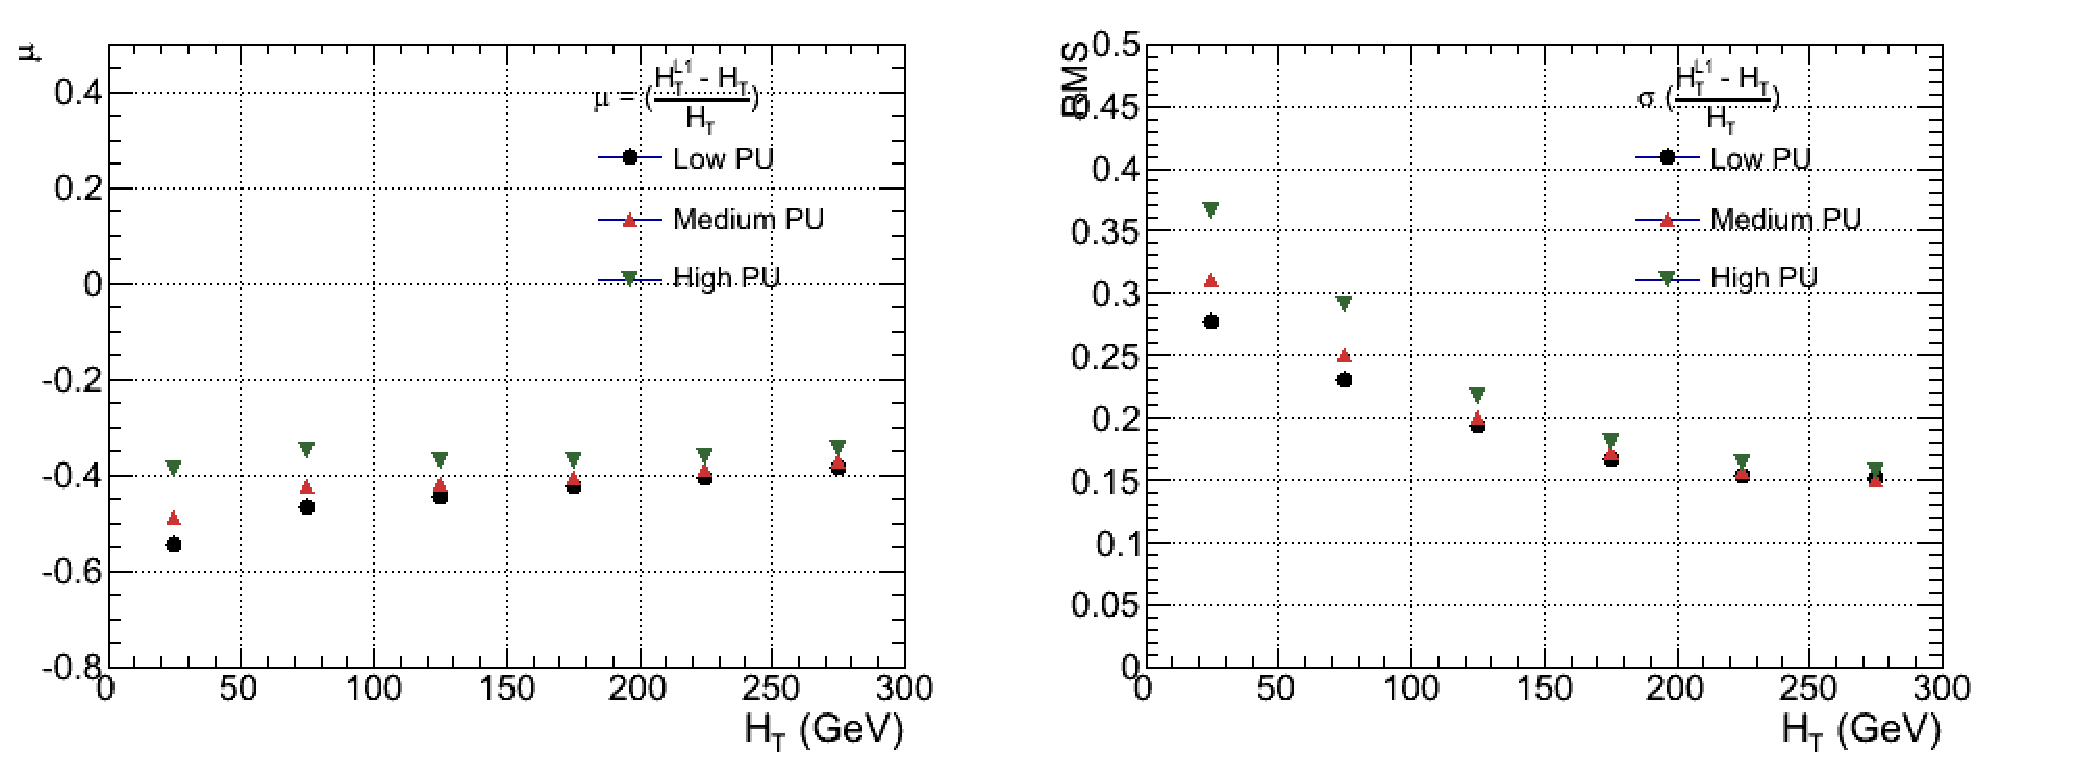
\includegraphics[width=1.0\textwidth]{plots/res_pfHT_summary.pdf}
        \caption[$\theht$~resolution parameters in bins of PF $\theht$~measured for the defined low, medium and high pile up conditions.]{$\theht$~resolution parameters in bins of PF $\theht$~measured for the defined low, medium and high pile up conditions. The plots show the mean $\mu$ (left), resolution $\sigma$ (RMS) of the $\frac{\Delta q}{q}$ distributions.}
        \label{fig:pfhtresultspu}
\end{figure}

\begin{figure}[h!]
  \vspace{20pt}
        \centering
        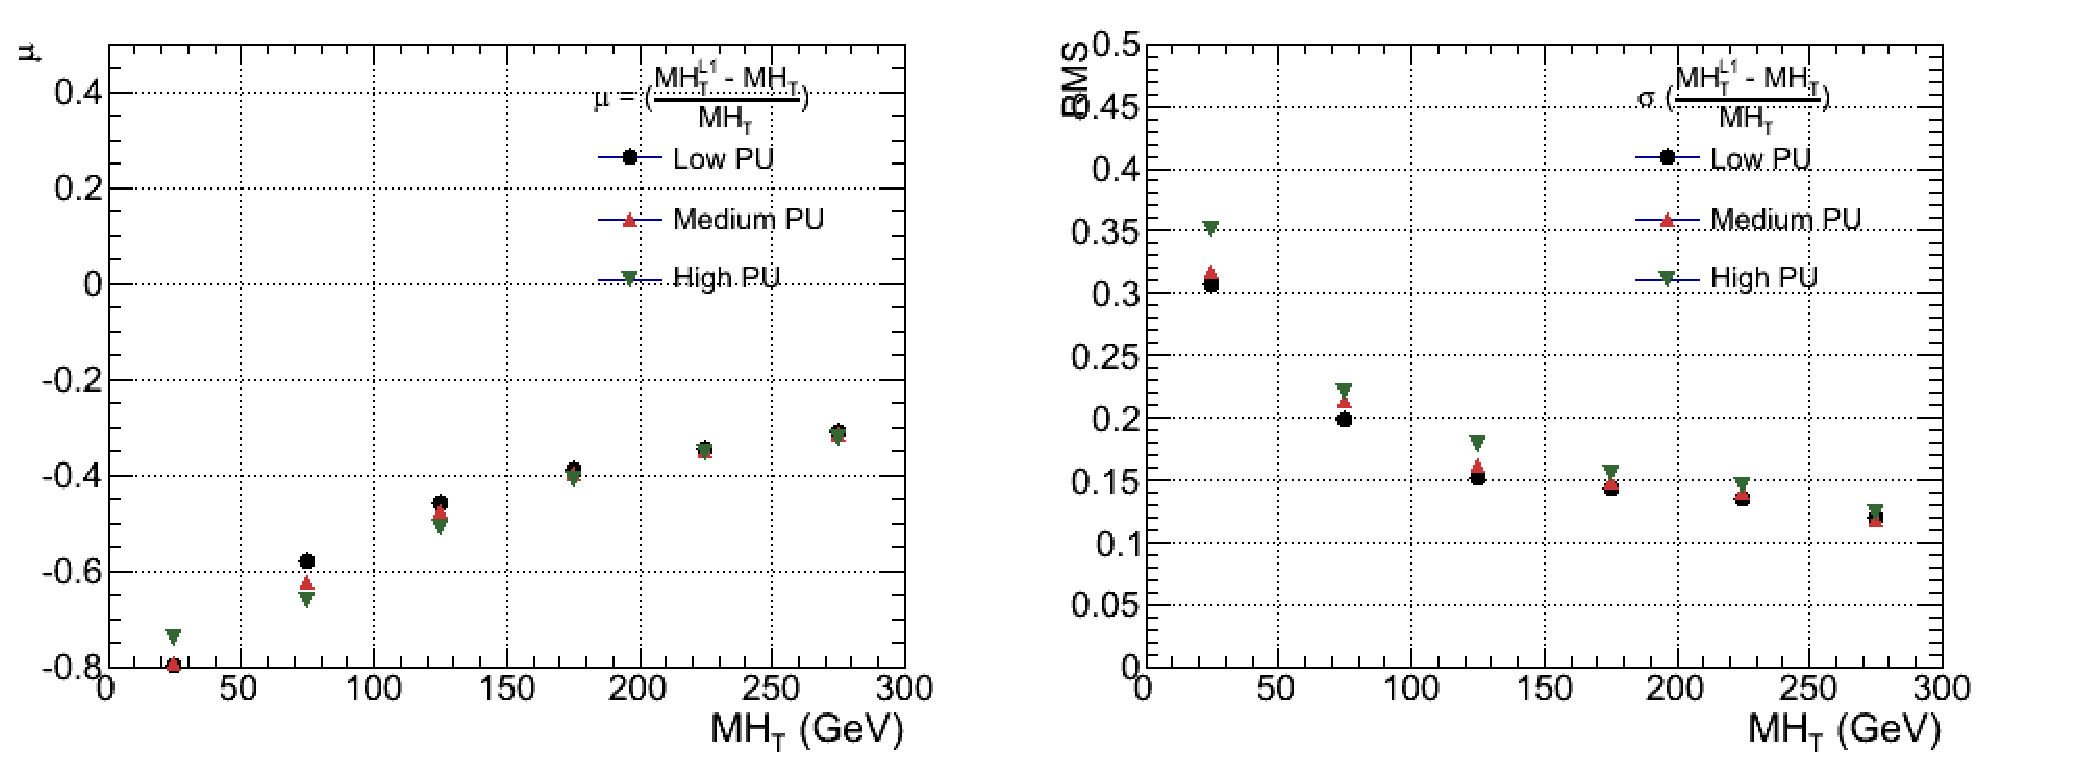
\includegraphics[width=1.0\textwidth]{plots/res_CaloMHT_summary.pdf}
        \caption[$\mht$~resolution parameters in bins of $\mht$~measured for the defined low, medium and high pile up conditions.]{$\mht$~resolution parameters in bins of $\mht$~measured for the defined low, medium and high pile up conditions. The plots show the mean $\mu$ (left), resolution $\sigma$ (RMS) of the $\frac{\Delta q}{q}$ distributions.}
        \label{fig:calomhtresultspu}
\end{figure}
\begin{figure}[h!]
  \vspace{20pt}
        \centering
        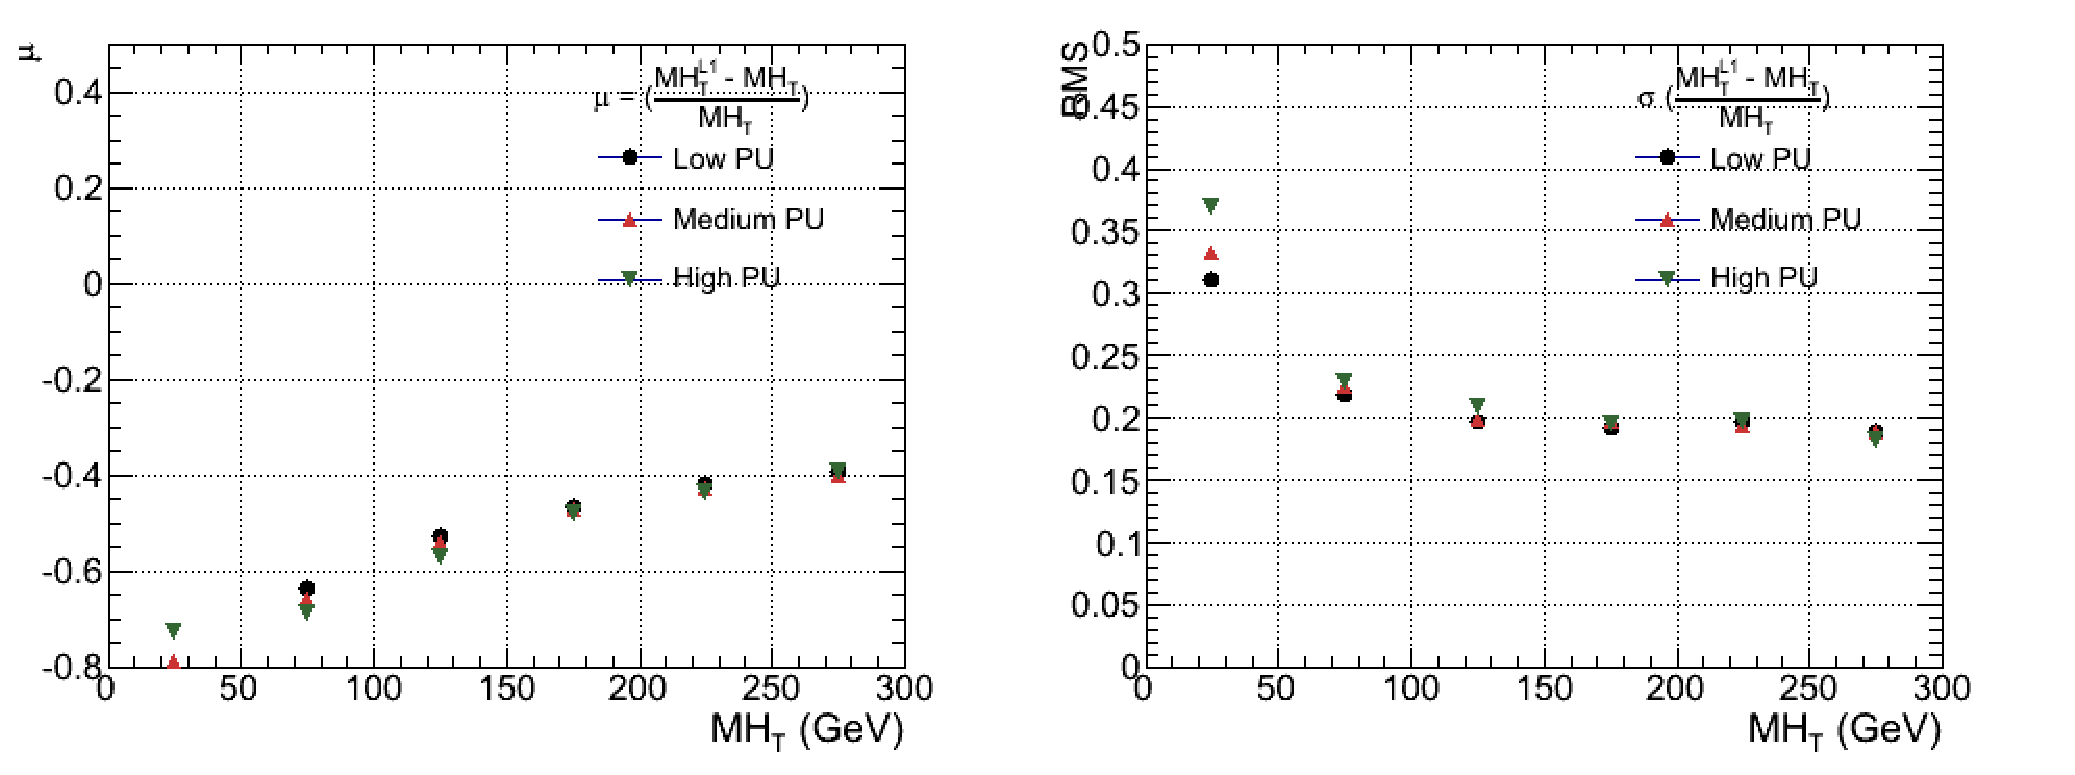
\includegraphics[width=1.0\textwidth]{plots/res_pfMHT_summary.pdf}
        \caption[$\mht$~resolution parameters in bins of PF $\mht$~measured for the defined low, medium and high pile up conditions.]{$\mht$~resolution parameters in bins of PF $\mht$~measured for the defined low, medium and high pile up conditions. The plots show the mean $\mu$ (left), resolution $\sigma$ (RMS) of the $\frac{\Delta q}{q}$ distributions.}
        \label{fig:pfmhtresultspu}
\end{figure}

\chapter{Additional material on background estimation methods}
\label{app:backgroundestimation}
\section{Determination of $k_{QCD}$}
\label{app:kqcd}


\begin{minipage}{\linewidth}
\centering
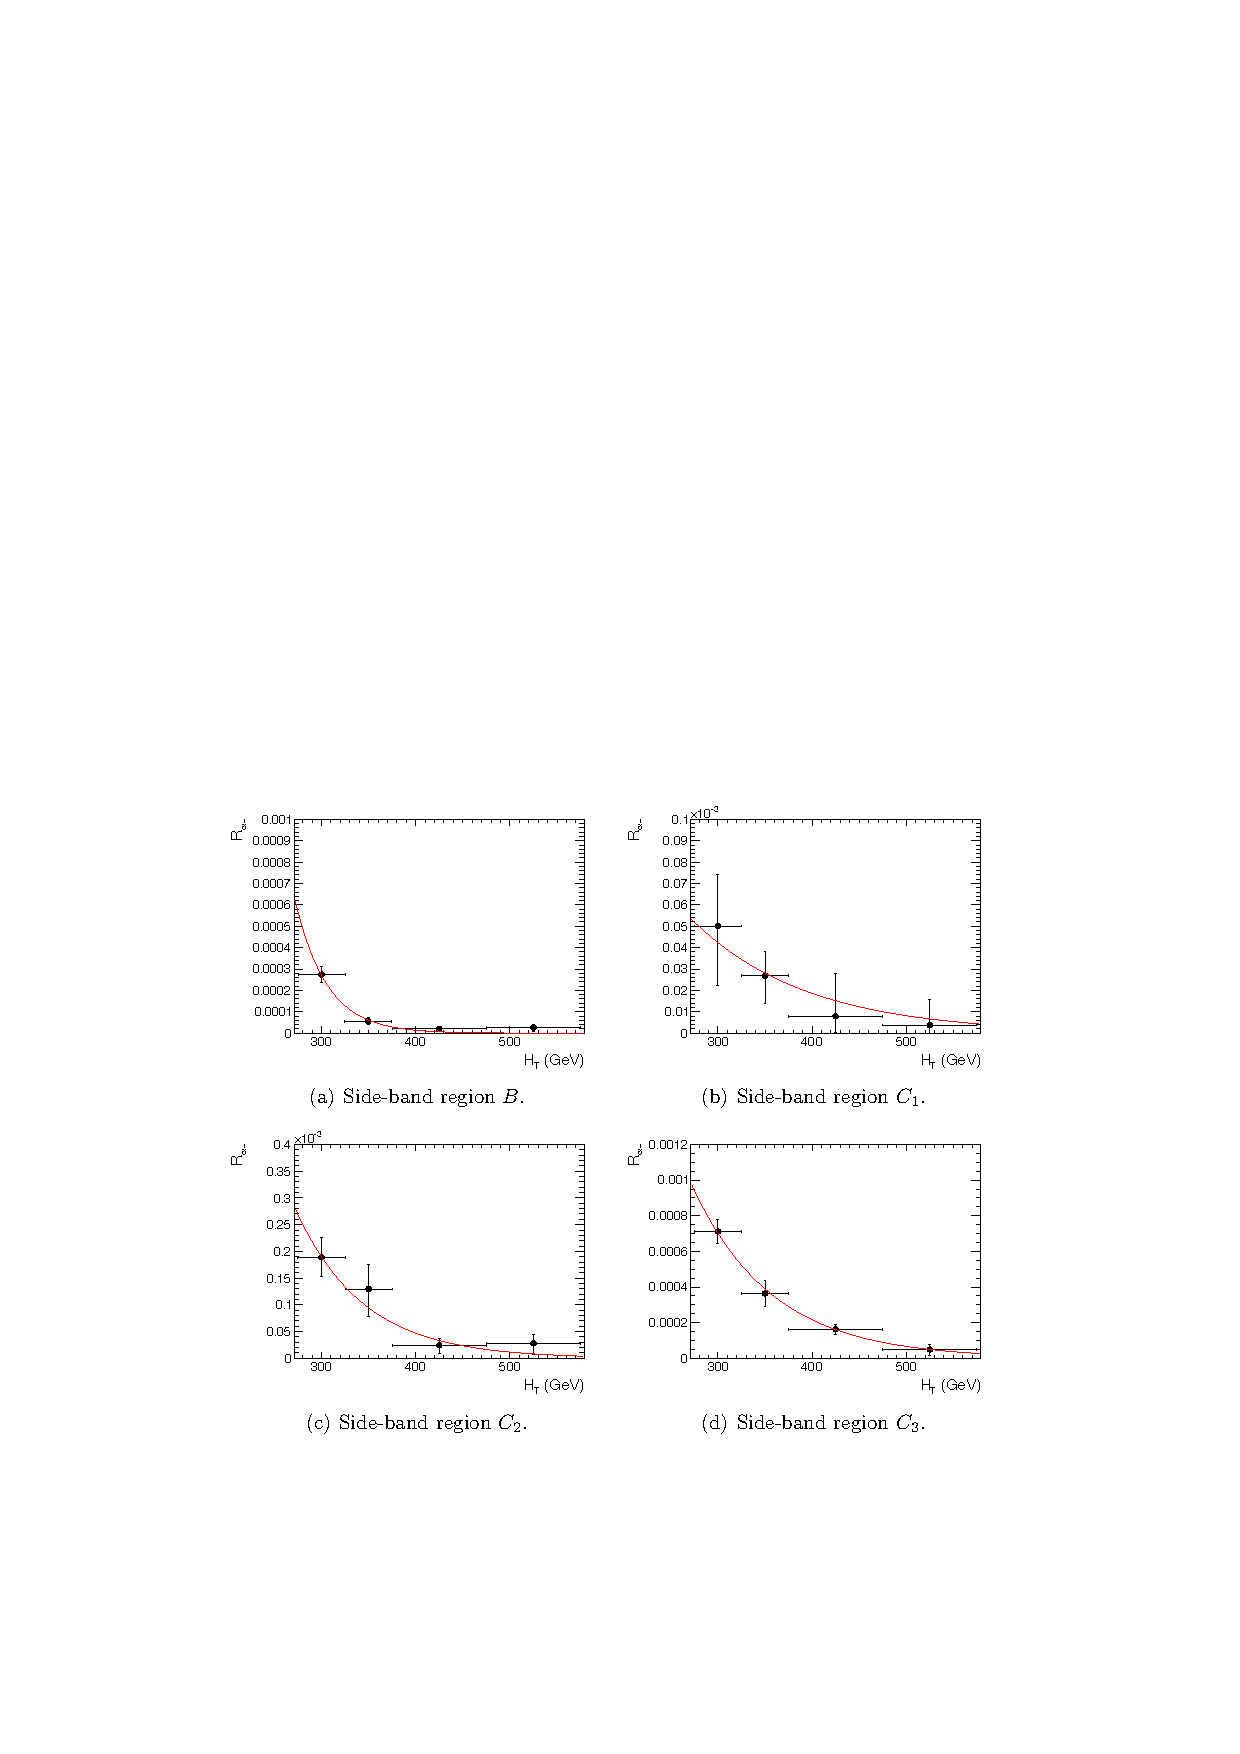
\includegraphics[width = 4.9in]{plots/qcd_sideband_fits.pdf}
\captionof{figure}[$R_{\alphat}$(\theht) and exponential fits for each of the data sideband regions. Fit is conducted between the \theht region 275 $<$ \theht $<$ 575.]{$R_{\alphat}$(\theht) and exponential fits for each of the data sideband regions. Fit is conducted between the \theht region 275 $<$ \theht $<$ 575.}
\label{fig:qcd_sideband_fits}
\end{minipage}


\section{Effect of varying background cross sections on closure tests }
\label{app:xsecvariation}

Closure tests with cross section variations of +20\% and -20\% applied to W + jets and \ttbar processes respectively.

\begin{figure}[ht]
\centering
\begin{minipage}[b]{0.48 \linewidth}
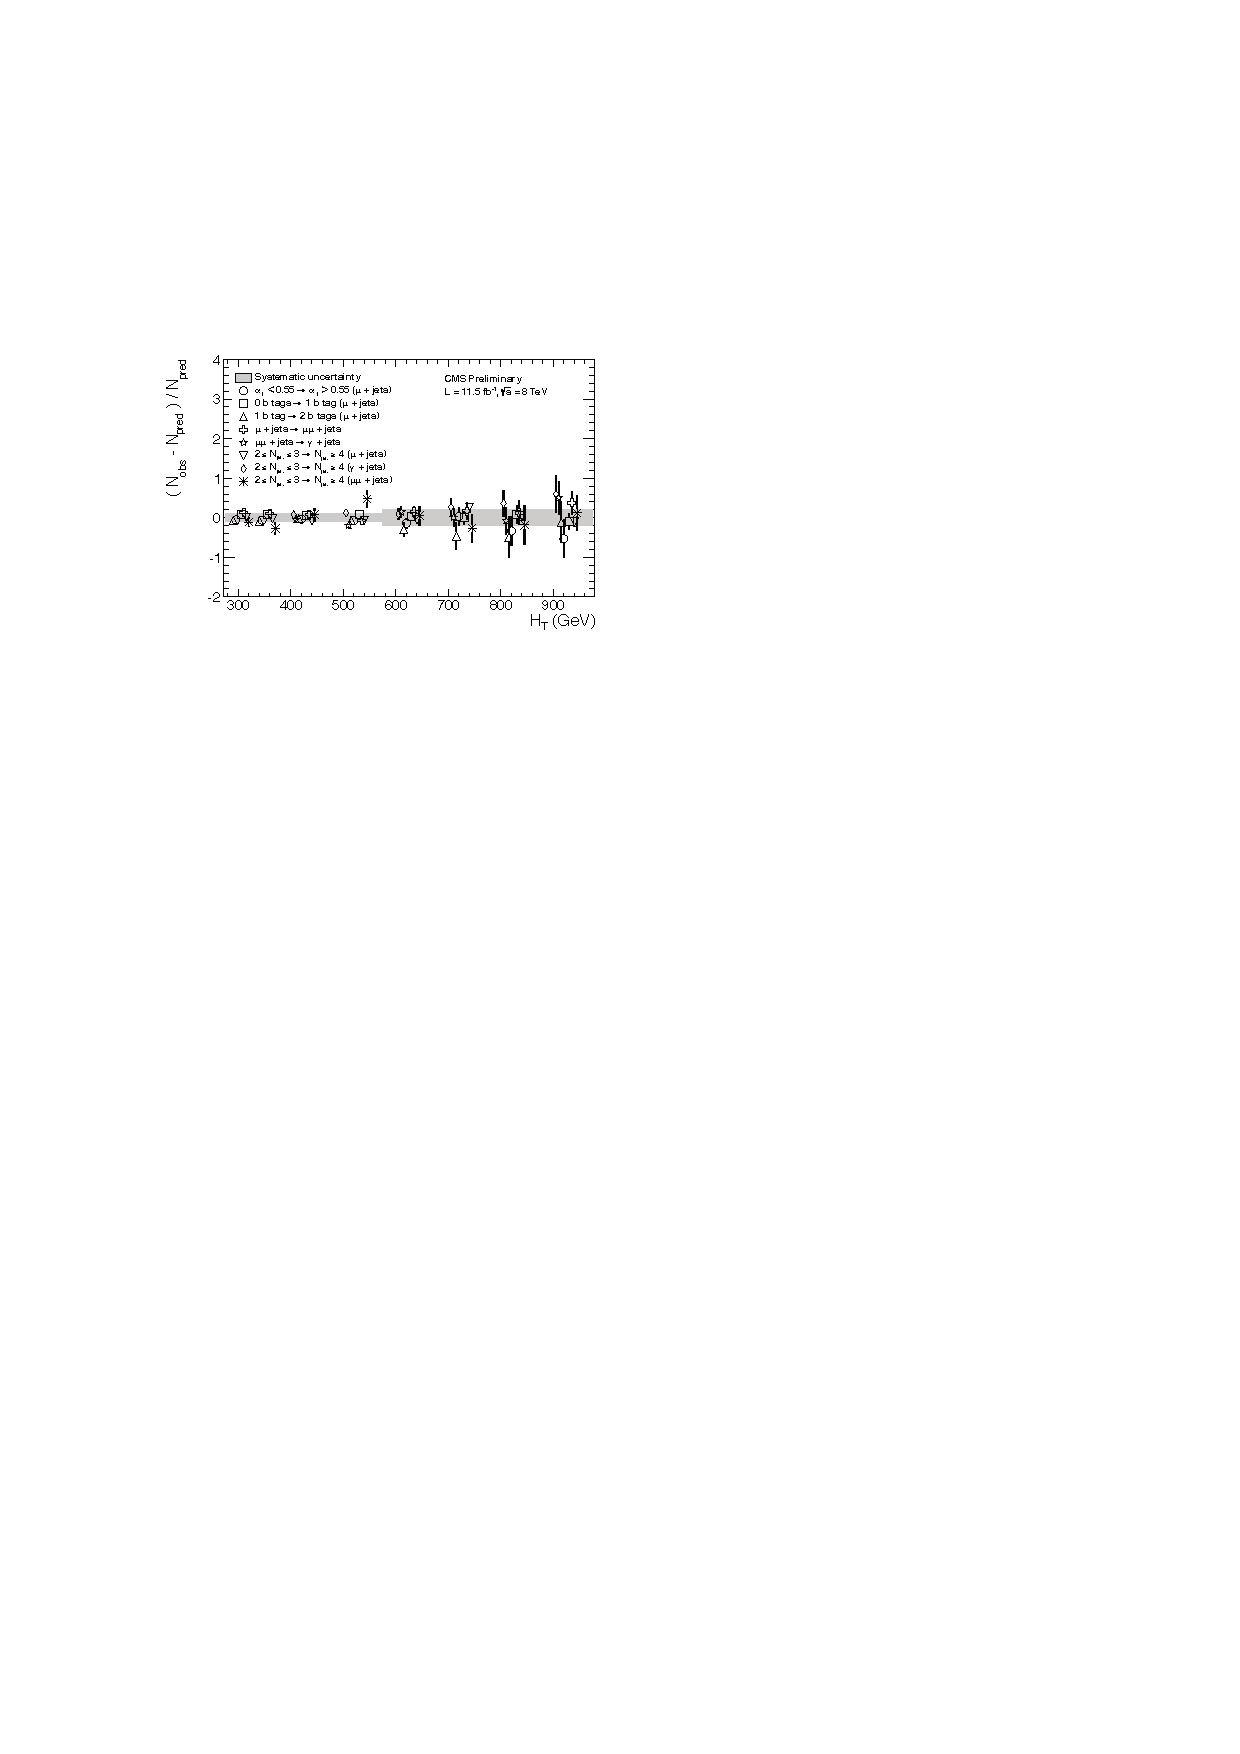
\includegraphics[width = 1.0\linewidth]{plots/syst-le3j_nominal.pdf}
\centering
(a)  
\end{minipage}
\quad
\begin{minipage}[b]{0.48\linewidth}
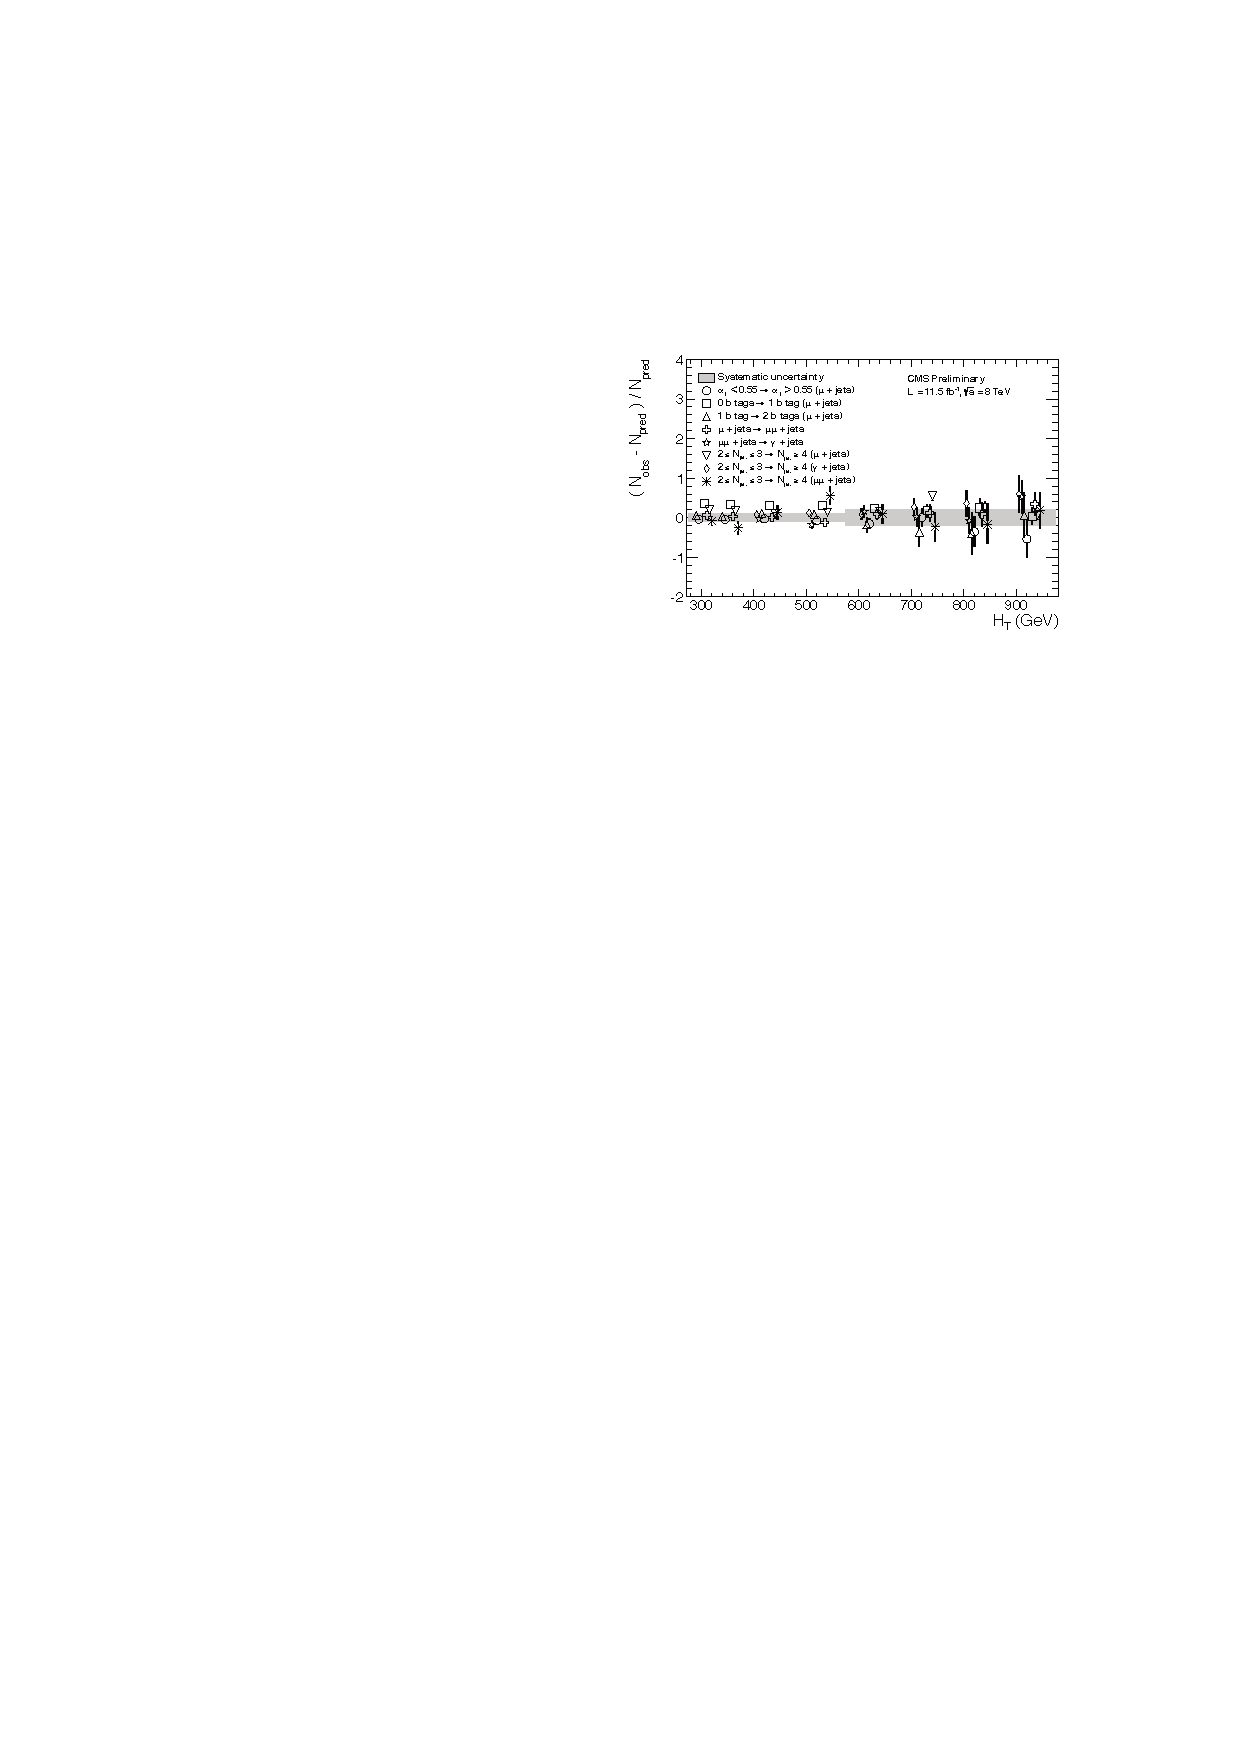
\includegraphics[width = 1.0\linewidth]{plots/syst-le3j_varied.pdf}
\centering
(b) 
\end{minipage}
\caption[Sets of closure tests overlaid on top of the systematic uncertainty used for each of the five \theht regions.]{Sets of closure tests (open symbols) overlaid on top of the systematic uncertainty used for each of the five \theht regions (shaded bands) and for the two different jet multiplicity bins:(a) $2 \leq n_{jet} \leq 3$ and (b) $n_{jet} \geq 4$.}
\label{fig:xsecvariedle3j}
\end{figure}


\begin{figure}[ht]
\centering
\begin{minipage}[b]{0.48 \linewidth}
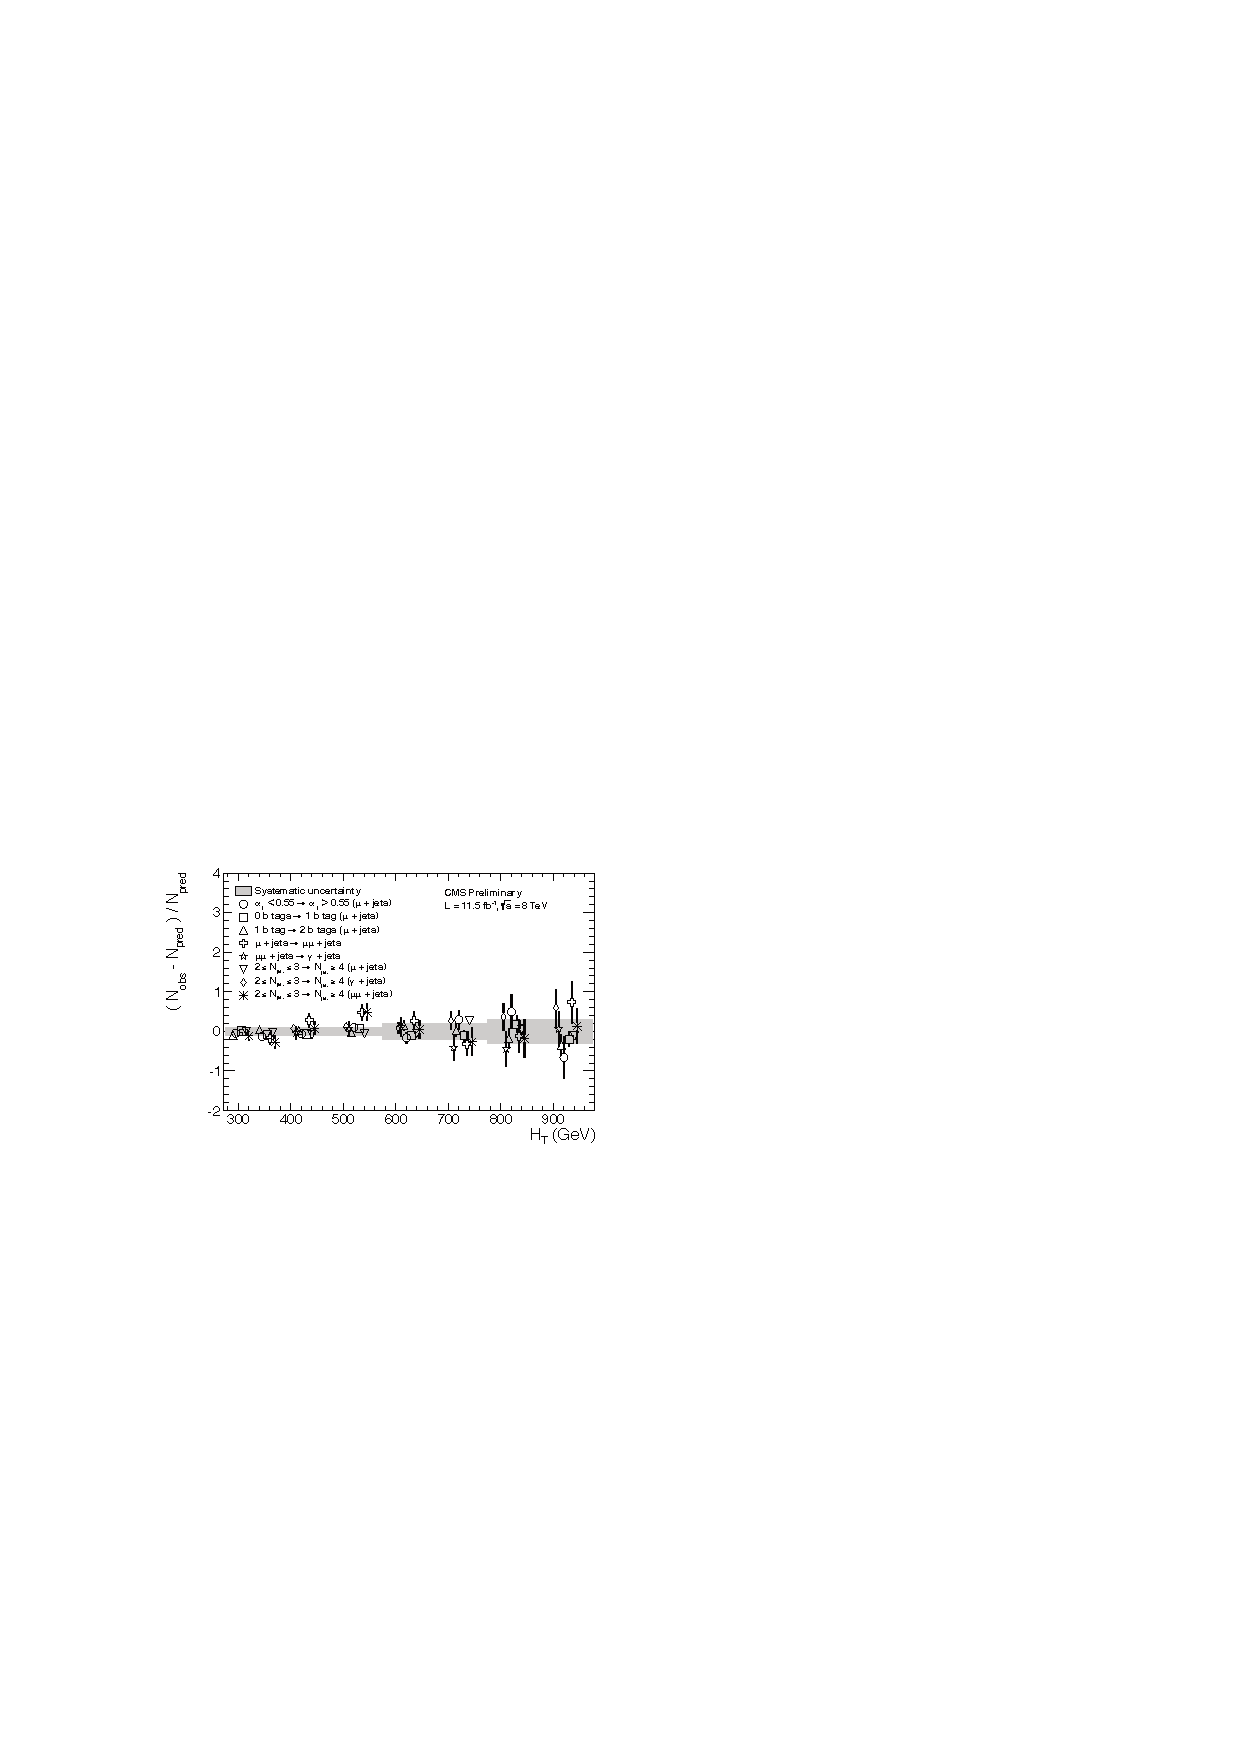
\includegraphics[width = 1.0\linewidth]{plots/syst-ge4j_nominal.pdf}
\centering
(a)  
\end{minipage}
\quad
\begin{minipage}[b]{0.48\linewidth}
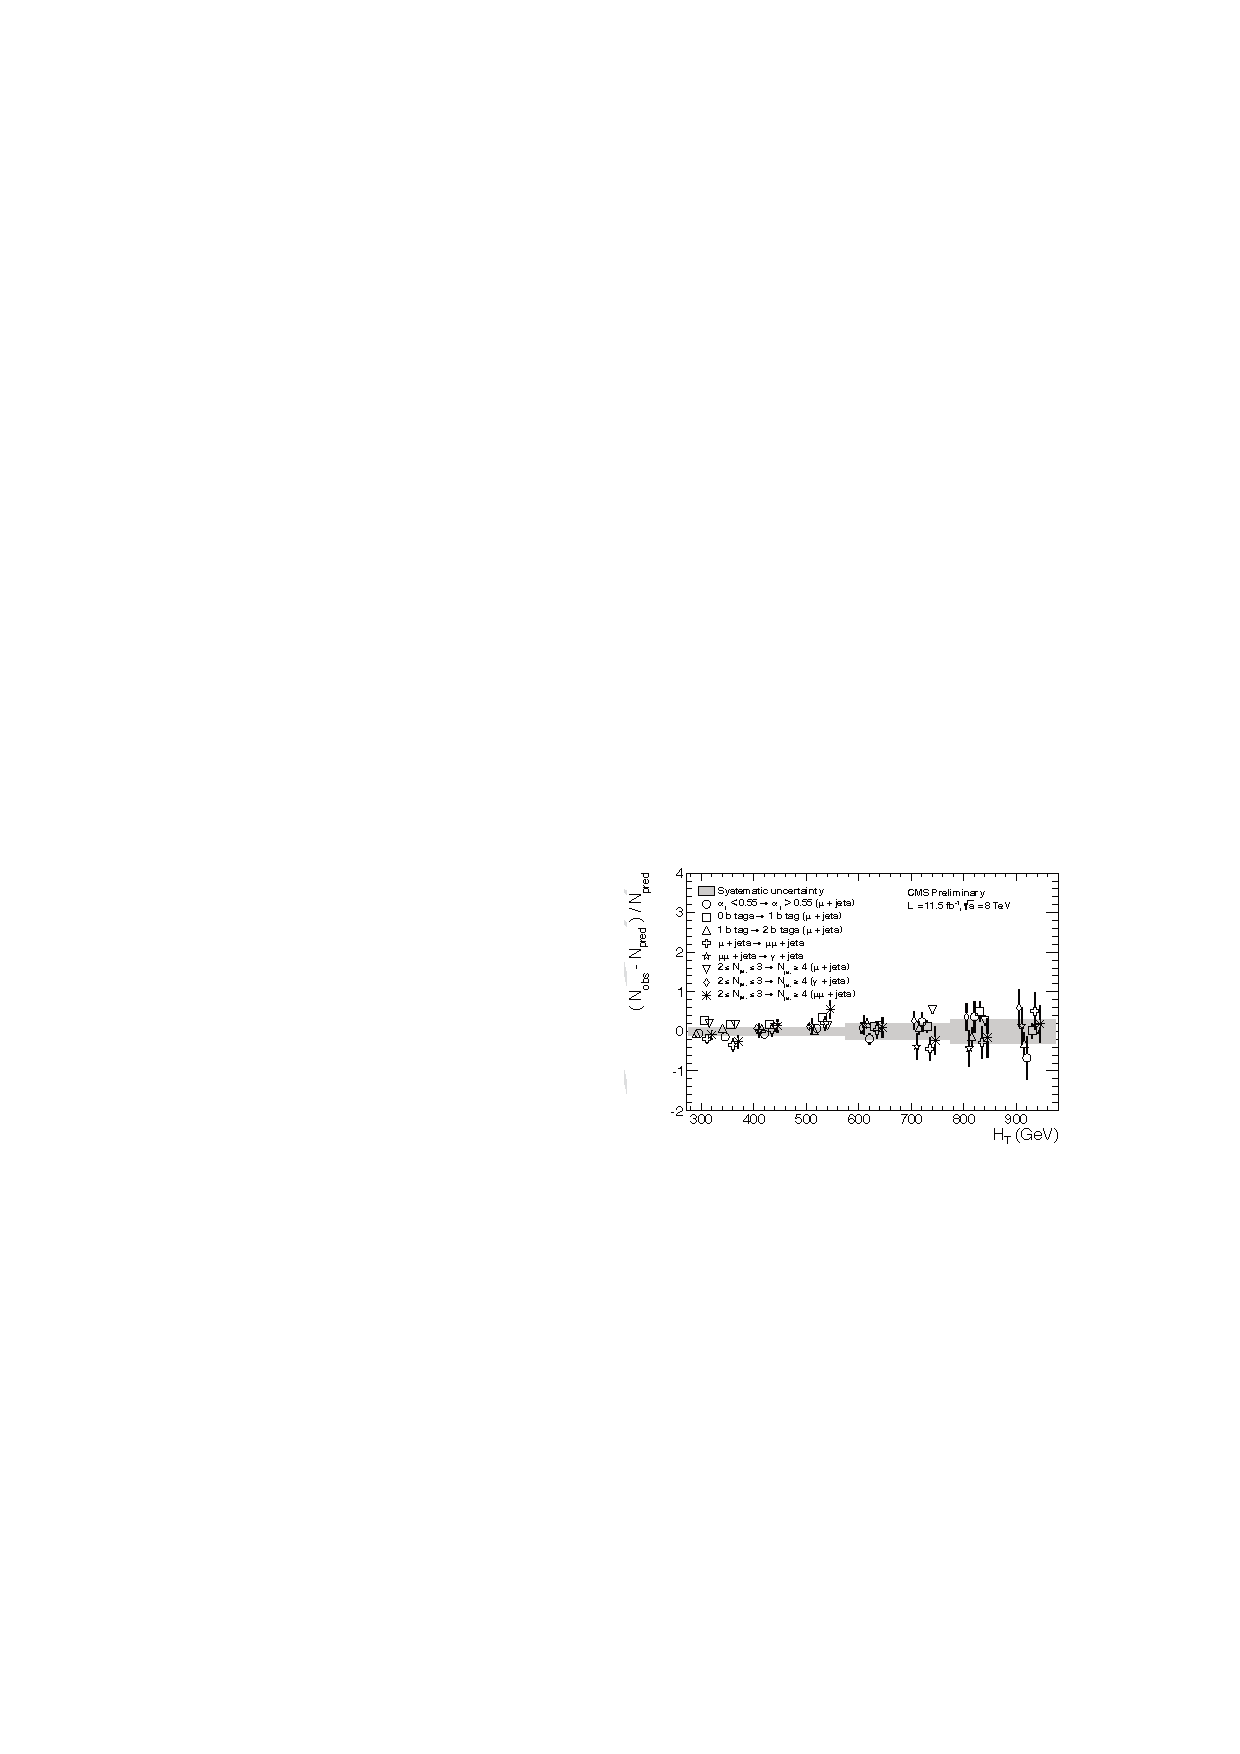
\includegraphics[width = 1.0\linewidth]{plots/syst-ge4j_varied.pdf}
\centering
(b) 
\end{minipage}
\caption[Sets of closure tests overlaid on top of the systematic uncertainty used for each of the five \theht regions.]{Sets of closure tests (open symbols) overlaid on top of the systematic uncertainty used for each of the five \theht regions (shaded bands) and for the two different jet multiplicity bins:(a) $2 \leq n_{jet} \leq 3$ and (b) $n_{jet} \geq 4$.}
\label{fig:xsecvariedge4j}
\end{figure}

 \begin{table}[h!]
\begin{center}
\begin{tabular*}{0.95\textwidth}{@{\extracolsep{\fill}}cl|cccc}
\cline{1-6}
&&\multicolumn{4}{l}{\theht (\GeV)} \\
\cline{1-6}
\cline{1-6}
\end{tabular*}
\end{center}
\caption[ ]{}\label{tab:xsecvaried}
\end{table}

